\documentclass[a4paper,11pt,oneside]{book}
\usepackage[T1]{fontenc}
\usepackage[utf8]{inputenc}
\usepackage{lmodern}
\usepackage{mathtools}
\usepackage{braket}
\usepackage{float}
\usepackage[backend=biber,sorting=none]{biblatex}
\addbibresource{references.bib}
\usepackage[bookmarks]{hyperref}

\makeatletter
\title{Investigation of Entanglement Measures in the Quantum Toolbox in Python (QuTiP)}  \let\Title\@title
\author{Muhammad Saad}                                \let\Author\@author
\newcommand{\supervisor}{Dr. Jamil Raza}
\date{Fall 2015}                                      \let\Date\@date
\makeatother


\hypersetup{
    pdftitle={\Title},
    pdfauthor={\Author},
    pdfsubject={Quantum Information Theory},
    pdfkeywords={qit, quantum, entanglement, quantum entanglement, quantum information, python},
    bookmarksnumbered=true,
    bookmarksopen=true,
    bookmarksopenlevel=1,
    %colorlinks=true,
    pdfstartview=Fit,
    pdfpagemode=UseOutlines,
    pdfpagelayout=TwoPageRight
}


\begin{document}

\begin{titlepage}
    \begin{center}
        \LARGE
        \textbf{\Title}\\
        \vspace{0.5cm}
        \LARGE
        Final year project for BS Physics\\
        \vspace{1.5cm}
        \Large
        Supervised by\\
        \supervisor\\
        \vspace{0.5cm}
        Submitted by\\
        {\Author}\\
        \large
        \vspace{0.8cm}
        \vfill
        
\includegraphics[width=0.4\textwidth]{title/iiui-logo.jpg}
        \vfill
        \Large
        Department of Physics\\
        Faculty of Basic and Applied Sciences\\
        International Islamic University, Islamabad\\
        \vfill
        \Date
    \end{center}
    
\end{titlepage}



\frontmatter
\chapter{Abstract}

During the last few decades considerable work has been done on quantum information theory with an emphasis on exploiting quantum entanglement. Various entanglement tests and measures have been devised to detect entanglement in experiments and quantify how much entanglement is contained within a system. This project implements some of these entanglement tests and measures in the Python programming language. We also implement some other quantum information related functions. We base our work on the library known as QuTiP (Quantum Toolbox in Python). Moreover, we provide practical examples of the new functions' usage through a number of simulations.


\chapter*{Acknowledgments}

This work would have been difficult to finish without the support of many people. I want to thank anyone who has lent a hand in the completion of this work in any way. Special thanks go to my supervisor Dr. Jamil Raza whose guidance and assistance helped a lot in the completion of this project. For me as someone completely new to the concepts of information theory, it was a great help. Thanks also to Syed Masood for his occasional help and continued moral support. I also want to thank my parents, siblings and friends especially Haseeb Hayat for their continuous moral support, and my teachers whose guidance throughout my life has made this possible.


\newpage
\phantomsection
\addcontentsline{toc}{chapter}{Contents}
\tableofcontents
\chapter{Overview of the Project}

\par The development of quantum mechanics in the early twentieth century introduced us to a whole new way of thinking about the universe. Moreover, it also introduced some extremely strange and non intuitive ideas. One such idea is the concept of non-locality. The phenomenon of quantum entanglement seemed so strange to the intellectual giants of that time, that they ended up calling it “spooky action at a distance”. Although later developments in quantum information theory showed this spooky action can be exploited for novel applications in communication. Today researchers are looking at quantum entanglement as an important resource in developing communication systems that nobody would have thought of fifty years earlier.
\par This project is primarily concerned with the phenomenon of quantum entanglement and the different ways to detect and quantify it. We have carried out some simulations of quantum information systems and implemented various tests and measures of quantum entanglement, along with some other quantum information functions, in the Quantum Toolbox in Python (QuTiP). Besides Python, we have also explored MATLAB and the quantum information toolboxes available for both of them.
\par In particular this project is concerned with \textit{adding} quantum information functionality to the QuTiP toolbox. QuTiP is an excellent simulator for open quantum systems but is currently lacking in terms of quantum information functionality. This project hopes to improves this. For now entanglement tests and measures are focused on more. In the future, this work can be extended to add even more QI functionality to QuTiP.
\par Here is a brief overview of this report.
\begin{enumerate}
  \item Chapter one introduces the basics of classical information theory.
  \item Chapter two provides a review of basic quantum mechanics.
  \item Chapter three extends the concepts of classical information theory to quantum information theory.
  \item Chapter four introduces the idea of computer simulations of physical systems and discusses some tools that we have available in the scope of this project. In this chapter we introduce MATLAB and Python, two popular programming languages in academia. We take a look at various toolboxes available for both to do quantum information simulations and research.
  \item Chapter five discusses the basics of QuTiP, an open quantum systems simulator for Python, and demonstrates how it can be used for solving quantum information problems.
  \item Chapter six explains in detail the code developed in this project. It details the implementation of the new quantum information functions in QuTiP, focusing mostly on entanglement tests and measures. It also demonstrates some basic simulations involving entangled states, applying the new functions and measures to them.
\end{enumerate}
We hope that this project will spark some interest in computational physics in our department and in the future more students will step forward to contribute in the development of more scientific programming libraries.



\mainmatter
\chapter{Fundamentals of Classical Information Theory}
\chaptermark{Classical Information Theory}

\par In 1948 Claude E. Shannon published the seminal article “A Mathematical Theory of Communication” exploring the problem of sending information over a communication channel. This was the concrete beginning of classical information theory. This chapter discusses the fundamental ideas of classical information theory. We discuss what information is, how efficiently it can be compressed or sent, and various measures to quantify information.

\par First we need to define exactly what we mean by the term “information”. Usually when people talk about information, they may have different meanings in mind. To some a literary work may have more information than a phone book, to others it may be the other way around. But to devise a formal theory of information we need to have a concrete and quantifiable definition of it.

\section{The Classical Bit}
\par Suppose we are holding an object. Let us ask a question: how much information is contained in this object? To answer the question, we'll have to think about a context in which we need to "transfer" that information to someone else. Let us say we have a friend to whom we need to transfer the complete information of this object. What would that information be? Information in this context will be the size of the set of instructions we need to provide that friend so that he can successfully reconstruct the object.
Suppose the object is an electrical switch and we need to send the information on what state the switch is in. The switch can have one of two possible states: on and off with equal probabilities. The information content we send will be a choice between these two possible alternatives. We call this binary choice a bit - or a binary digit.
\par In general, we can reduce a choice between any number of alternatives to $n$ number of choices between binary alternatives. If we need to make one binary choice between equally probable outcomes then the information content is said to be one bit. If we have to specify between $n$ number of such binary choices then we say the information content is $n$ bits.


\section{Quantifying Classical Information}
The \textit{bit} discussed earlier is a \textit{unit} for information. We now explore the \textit{quantity} - information itself - for which the bit is a unit. To do that we take a look at Shannon's original work on classical information theory.
\par Shannon in his work modeled information as events that happen with certain probabilities. To devise a measure of information he postulated some requirements which any measure of information must fulfill.
\begin{itemize}
\item The amount of information in an event $x$ must depend only upon its probability $p_x$ of happening. In this sense, events that are less likely to happen will carry more information than events that are more likely to happen. We can also say that information is the amount of surprise in an event.
\item Information $I(p)$ is a continuous function of $p$. As we are already familiar, continuity is indeed a desirable quality for physical quantities.
\item $I(p_x,p_y)=I(p_x)+I(p_y)$ which means that information contained in two independent events should be additive.
\end{itemize}
\par Shannon proved that there is indeed a unique measure of information which satisfies these requirements. This measure is unique upto an additive and multiplicative constant. This measure we call the \texttt{Shannon Entropy}.

\subsection{Shannon Entropy}
\par Suppose a message consists of a long string of letters in which each letter $i$ comes from a set of $n$ different letters, each occurring with a probability $p_i$. From requirement 1 it is clear that the information content of the message should depend on $1/p_i$. The less probable the letter, the more surprise you have. To fulfill requirement 3 we choose the function $\log$. Thus the information $I(i)$ in one of the letters $i$ is
\begin{align*}
I(i) = \log\frac{1}{p_i}
\end{align*}
We can see that if we have two events (or two letters), the surprise is additive.
\begin{align*}
I(i,j)= \log(\frac{1}{p_i}\frac{1}{p_j}) = \log\frac{1}{p_i} + \log\frac{1}{p_j}
\end{align*}
The average information contained in a message is the \textbf{Shannon Entropy}.
\begin{align*}
H = \sum_i p_i \log \frac{1}{p_i} = - \sum_i p_i \log p_i
\end{align*}

\subsection{Data Compression}
\par The basic concept of data compression is based on the idea that in any given message there will be redundancy of certain letters or symbols used to encode that message. Such redundancy can always be eliminated by encoding the message more efficiently. In this section we explore the minimum theoretical limit to which we can compress a given message.
\par Suppose we have a long message comprising of a large number $N$ of binary letters. As $N$ gets large enough, $N p_1$ of these letters will be 1's and $N p_0$ letters will be 0's. The number of ways we can arrange these letters is
\begin{align*}
\frac{N!}{(N p_1)!(N p_o)!}
\end{align*}
which are all equally likely to occur.
\par We can label all of them with a binary number. The number of binary digits $I$ we will need to label all these is
\begin{align*}
I = \log_2 (\frac{N!}{(N p_1)!(N p_o)!})
\end{align*}
For a large enough message the original $N$ bits message can be reconstructed with arbitrary precision using just $I$ bits.
Using Stirling's approximation for log of factorials
\begin{align*}
\log(M!) = M \log(M) - M
\end{align*}
We get the relation for information content $I$ of the message
\begin{align*}
I = -N ( p_1 \log p_1 + p_0 \log p_0 )
\end{align*}
which can be generalized to $i$ letters each occurring with probability $p_i$. When we sum them up, we find the familiar expression for Shannon entropy which now also relates to the average information content per symbol.
\begin{align*}
\frac{I}{N} = H\{p_i\} = - \sum_{i=1}^{n} p_i \log p_i
\end{align*}

\section{Capacity of a Noisy Channel}
\par Let's say Alice wants to send Bob a message over a classical information channel. If the channel is noisy then there is a chance that some bits that Alice sends will be flipped and change their original state.

\begin{figure}[h]
  \begin{center}
    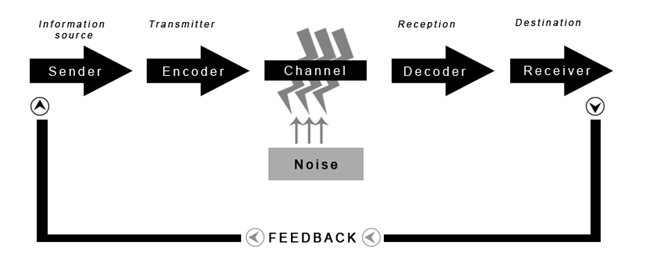
\includegraphics[scale=0.58]{figures/shannon-model-of-communication.png}
    \caption{Shannon's model of communication. A sender encodes some message and transmits it through a channel whereby a receiver receives it and decodes it to access the information that was encoded. Along the channel may exist a source of noise which disrupts the message that was originally sent.}
    \label{fig:}
  \end{center}
\end{figure}

\par We can think of the process like this. What Alice sends is a random variable $X$ and information encoded in that variable. What Bob receives at his end is another random variable $Y$, which depends on both the distribution $X$ and external factors (noise). The information Bob can get out of measuring $Y$ is the mutual information between $X$ and $Y$, $I(X:Y)$. This mutual information is the capacity of that noisy channel. The limit on this capacity is given by Shannon's noisy channel coding theorem.

\subsection{Shannon's Noisy Channel Coding Theorem}
\par If $R$ is the rate of information production and $C$ is the channel capacity, then the information can be transmitted over a noisy channel with arbitrary reliability if
\begin{align*}
R<C=I(X:Y)
\end{align*}
\par If we choose a source that produces information at a greater rate than the channel capacity, then the channel will be unable to handle the information reliably and errors will be inevitable.


\chapter{Quantum Mechanics: The Basics}

This chapter is a brief review of the fundamental quantum mechanics necessary for our treatment of quantum information theory. In here we discuss the basic mathematical objects and tools we shall deal with in the next chapter.

\section{Representing a Quantum Mechanical State}
\par The quantum mechanical state of a system is represented by a vector $\Ket{\psi}$ in the complex vector space known as the Hilbert space. In this section we see how such a state is constructed.
\par Let us consider a two-level quantum system such as a spin-half particle. Its state can be written in terms of two basis states which represent spin-up and spin-down. We can call these basis states $\Ket{0}$ and $\Ket{1}$ which are two orthogonal and normalized vectors in the Hilbert space.
\begin{align*}
\Ket{0} = \left(\! \begin{array}{c} 1 \\ 0 \end{array} \!\right) \\
\Ket{1} = \left(\! \begin{array}{c} 0 \\ 1 \end{array} \!\right)
\end{align*}
In such case the general state of the particle can be written as
\begin{align*}
\Ket{\psi} = \alpha \Ket{0} + \beta \Ket{1}
\end{align*}
\par When the particle's spin along an axis is measured, it collapses to one of these two states $\Ket{0}$ and $\Ket{1}$ with probabilities $|\alpha|^2$ and $|\beta|^2$ respectively with the condition that
\begin{align*}
|\alpha|^2 + |\beta|^2 = 1
\end{align*}
\par Instead of the basis states chosen above we could have chosen any other other as long as they are orthogonal and normalized so that they represent perfectly distinguishable outcomes in an experiment. One such example would be
\begin{center}
$ \frac{1}{\sqrt{2}} \left(\! \begin{array}{c} 1 \\ 1 \end{array} \!\right) $ and $ \frac{1}{\sqrt{2}} \left(\! \begin{array}{c} -1 \\ 1 \end{array} \!\right) $
\end{center}
The important point is that the chosen basis has to be consistent across our calculations. That is, when we bring physical quantities together in a calculation they have to be represented in the same basis. If they are not then they will need to be rotated into one standard basis. This operation of rotation is called a unitary transformation and represented by a matrix $U$ such that $U U^\dagger = U^\dagger U = I$. Unitary transformations have the property that they do not change the physically observable outcomes. Under a unitary transformation the predictions for all those observables will remain the same.
\par After establishing the general idea let us now look at an example state we may represent in this way.
\begin{align*}
  \Ket{\psi} &= \frac{2}{\sqrt{5}} \Ket{0} + \frac{1}{\sqrt{5}} \Ket{1} \\
  &= \frac{2}{\sqrt{5}} \left(\! \begin{array}{c} 1 \\ 0 \end{array} \!\right) + \frac{1}{\sqrt{5}} \left(\! \begin{array}{c} 0 \\ 1 \end{array} \!\right) \\
  &= \frac{1}{\sqrt{5}} \left(\! \begin{array}{c} 2 \\ 1 \end{array} \!\right)
\end{align*}
\par In this case we see that $\alpha = \frac{2}{\sqrt{5}}$ and $\beta = \frac{1}{\sqrt{5}}$.
\section{Pure States and Mixed States}
In terms of information that we have about the preparation of a quantum mechanical state, we identify it as either a pure state or as a mixed state.
\subsection{Pure State}
\par A pure state is a state for which we have complete knowledge about the preparation procedure. We already know in advance how the state was prepared, which, in principle is all that we can know about the system. The example of $\Ket{\psi}$ in the previous section is that of a pure state. We have a single state $\Ket{\psi}$ with 100\% certainty and the predictions we can make about it can be no more accurate than they are with our current knowledge of it.
\par At this point it will be appropriate to introduce a more general representation of a quantum mechanical state than a simple ket vector. This representation we are going to introduce is called the \textbf{density operator or density matrix}.
\subsection{The Density Operator}
\par The density operator for a state $\Ket{\psi}$ is simply a projection operator that projects all the vectors onto the state vector $\Ket{\psi}$.
\par If $\Ket{\psi}$ is represented by the column vector
\begin{align*}
\Ket{\psi} = \left(\! \begin{array}{c} a \\ b \end{array} \!\right)
\end{align*}
Then the density operator for the state would be
\begin{align*}
  \hat{\rho} = \Ket{\psi} \Bra{\psi} &= \begin{pmatrix} a \\ b \end{pmatrix} \begin{pmatrix} a^* & b^* \end{pmatrix} \\
  &= \begin{pmatrix} |a|^2 & a b^* \\ a^* b & |b|^2 \end{pmatrix}
\end{align*}
\par From this density operator we can determine outcomes of physical experiments. In quantum mechanics physical observable quantities are represented by Hermitian operators. Suppose we apply an observable $\hat{O}$ to the density matrix which is the mathematical equivalent of performing the observation in an experiment. The state will collapse and the outcome of the experiment will have the expectation value of
\begin{align*}
  \braket{\hat{O}} &= tr\{\hat{O} \Ket{\psi} \Bra{\psi}\} \\
  \braket{\hat{O}} &= tr\{\hat{O} \hat{\rho}\}
\end{align*}
Here $tr$ represents the trace operation, which is taking the sum of all entries on the main diagonal of the matrix.

\subsection{Mixed State}
\par In general when we deal with quantum systems in the real world, we will not have complete knowledge on how the state was prepared. This lack of knowledge can be due to several factors. It can be caused by errors in the apparatus that prepares the quantum state or it can be introduced later by environmental factors. In both cases we will not have a pure state with 100\% certainty.
\par Let us take a look at a real world example. Suppose we want to prepare a number of atoms in state $\ket{\psi_0}$. We have an apparatus to do that for us. However due to some random error in the machinery some of the atoms are prepared in state $\ket{\psi_1}$ instead. Let's suppose the state we want, $\ket{\psi_0}$, is prepared with a 95\% accuracy. Then the rest of the atoms we get from the machine - 5\% of them - will be in state $\ket{\psi_1}$. In this case we have a mixed state.
\par Notice that the probabilities involving the states are no longer limited to the quantum domain. There are now classical probabilities involved as well. 0.95 is the classical probability of $\ket{\psi_0}$ occurring in the mix and 0.05 is the classical probability of $\ket{\psi_1}$ occurring.
\par In general, we will have a mixture of more than one states each occurring with its respective classical probability. $\ket{\psi_0}$ with probability $p_0$, $\ket{\psi_1}$ with probability $p_1$, $\ket{\psi_2}$ with probability $p_2$, and so on.

\subsection{Density Operator for Mixed States}
\par For a mixture of a number of quantum states where each state $\ket{\psi_i}$ occurs with classical probability $p_i$, the density operator is written as
\begin{align*}
\hat{\rho} = \sum_i \ket{\psi_i} \bra{\psi_i}
\end{align*}
\par As we saw in the case of pure states, expectation values for experimental outcomes are calculated in a similar fashion. If $\hat{O}$ is the operator representing the observable quantity, then the expectation value for the operator will be given by
\begin{align*}
\braket{\hat{O}} = tr\{\hat{O}\hat{\rho}\}
\end{align*}
\par Similarly, we can calculate the probability of finding the system in a state $\ket{\sigma}$ by constructing the projection operator for that state $\ket{\sigma} \bra{\sigma}$ and applying it to the density operator $\hat{\rho}$ representing our system.
\begin{align*}
Prob_{\ket{\sigma}} = tr\{ \ket{\sigma} \bra{\sigma} \hat{\rho} \}
\end{align*}

\subsection{Basic properties of the density operator}
\par For a physically realizable state the density operator will always have the properties that
\begin{enumerate}
  \item It will be Hermitian
  \item It will have trace 1:
  $ tr\{\hat{\rho}\} = 1 $
\end{enumerate}
\par There is another additional property that will help us differentiate between density matrices for pure states and mixed states.
\begin{itemize}
  \item For a pure state, $ tr\{ \hat{\rho}^2 \} = 1 $
  \item For a mixed state, $ tr\{ \hat{\rho}^2 \} < 1 $
\end{itemize}

\section{Joint State of two Systems}
\par So far we have dealt with quantum mechanical states of isolated particles. What will happen if we consider the joint state of more than one such particles? Classical intuition says that the joint state consisting of two subsystems A and B at any time can be completely specified simply by specifying the states of A and B individually. It turns out that this idea does not always work in the domain of quantum mechanics. In quantum mechanics, the joint state of two or more subsystems is specified by their \textit{tensor product}. Let us take a look at a simple example to get some understanding of tensor products and joint states.
\par Suppose we have two atoms whose states are specified by $\ket{\psi_A}$ and $\ket{\psi_B}$.
\begin{align*}
  \ket{\psi_A} = \begin{pmatrix} a \\ b \end{pmatrix} \\
  \ket{\psi_B} = \begin{pmatrix} c \\ d \end{pmatrix}
\end{align*}
The joint state for $\ket{\psi_A}$ and $\ket{\psi_B}$ will be represented by the tensor product
\begin{align*}
  \ket{\psi_{AB}} &= \ket{\psi_A} \otimes \ket{\psi_B} \\
                &= \begin{pmatrix} a \\ b \end{pmatrix} \otimes \begin{pmatrix} c \\ d \end{pmatrix} \\
                &= \begin{pmatrix} ac \\ ad \\ bc \\ bd \end{pmatrix}
\end{align*}
Tensor products for higher dimensional vectors are obtained by component-wise multiplication in a similar fashion.
\par Let us now take a look at a simple example for joint state of two atoms where atom A is in the ground state $\ket{0}$ and atom B is in the excited sate $\ket{1}$. The joint state of both particles will be
\begin{align*}
  \ket{\psi_{AB}} &= \ket{0}_A \ket{1}_B \\
                  &= \begin{pmatrix} 0 \\ 1 \\ 0 \\ 0 \end{pmatrix}
\end{align*}
\par This suggests a more compact way of writing a joint state of two particles in our extended four-dimensional Hilbert space.
\begin{align*}
  \ket{\psi_{AB}} &= ac \ket{0}_A \ket{0}_B + ad \ket{0}_A \ket{1}_B + bc \ket{1}_A \ket{0}_B + bd \ket{1}_A \ket{1}_B 
\end{align*}
where the four basis vectors represent possible combinations of ground and excited states of atoms A and B and the corresponding co-efficients squared are the probabilities of finding that particular combination. For example, $|ad|^2$ is the probability of the state collapsing to atom A in ground state and atom B in excited state. 

\subsection{Operators for Joint States}
\par We have seen how joint states of two particles are given by tensor products which extend the systems to a higher dimensional Hilbert space. In our example two particles in their respective two-dimensional Hilbert spaces were extended to a four-dimensional Hilbert space. That means that the operators that work on those states will also be 4x4 matrices in the 4-D Hilbert space.
\par Suppose $\hat{O}_A$ and $\hat{O}_B$ are different observables acting respectively on the Hilbert space of particle A and particle B. The joint observable will be a tensor product of the two.
\begin{align*}
  \hat{O}_{AB} &= \hat{O}_A \otimes \hat{O}_B \\
               &= \begin{pmatrix} a_1 & b_1 \\ c_1 & d_1 \end{pmatrix} \otimes \begin{pmatrix} a_2 & b_2 \\ c_2 & d_2 \end{pmatrix} \\
               &= \begin{pmatrix} 
                    a_1 a_2 & a_1 b_2 & b_1 a_2 & b_1 b_2 \\
                    a_1 c_2 & a_1 d_2 & b_1 c_2 & b_1 d_2 \\
                    c_1 a_2 & c_1 b_2 & d_1 a_2 & d_1 b_2 \\
                    c_1 c_2 & c_1 d_2 & d_1 c_2 & d_1 d_2
                  \end{pmatrix}
\end{align*}
\par As a simple exercise let us construct a projection operator for projecting atom A on its ground state and atom B on its excited state. The isolated projector for A in this case is $\ket{0} \bra{0}$ and for B it is $\ket{1} \bra{1}$. The joint projector will be a tensor product of the two.
\begin{align*}
  \ket{0} \bra{0} \otimes \ket{1} \bra{1} &= \begin{pmatrix} 1 & 0 \\ 0 & 0 \end{pmatrix} \otimes \begin{pmatrix} 0 & 0 \\ 0 & 1 \end{pmatrix} \\
  &= \begin{pmatrix} 0 & 0 & 0 & 0 \\ 0 & 1 & 0 & 0 \\ 0 & 0 & 0 & 0 \\ 0 & 0 & 0 & 0 \end{pmatrix}
\end{align*}
\par We can apply this joint projection operator to a density operator for a joint state in a 4-D Hilbert space and take the trace to find out the probability for the outcome where A is in $\ket{0}$ and B is in $\ket{1}$.

\subsection{Partial Trace and the Reduced Density Operator}
\par Just like the example of joining two operators to form a combined operator in the enlarged Hilbert space, we can also take the tensor product of two density operators (or density matrices) to form the combined density operator for two particles A and B.
\begin{align*}
\hat{\rho}_{AB} = \hat{\rho}_A \otimes \hat{\rho}_B
\end{align*}
\par But what if we needed to do the inverse? Sometimes we will have a situation where we need to find the density matrix $\hat{\rho}_A$ from a combined density matrix $\hat{\rho}_{AB}$. The mathematical operation for that is called a partial trace over B and is denoted by
\begin{align*}
\hat{\rho}_A = tr_B\{ \hat{\rho}_{AB} \}
\end{align*}
We trace out system B and are left with only system A.
\par For a 4x4 density matrix, the partial trace over B to get the 2x2 density matrix for A looks like this.
\begin{align*}
\begin{pmatrix} a & b & c & d \\ e & f & g & h \\ i & j & k & l \\ m & n & o & p \end{pmatrix}
\rightarrow
\begin{pmatrix} a+f & c+h \\ i+n & k+p \end{pmatrix}
\end{align*}

\section{Entangled States}
\par In the previous section, we saw how we can write the product state of two particles as
\begin{align*}
\ket{\psi_{AB}} = ac \ket{0}_A \ket{0}_B + ad \ket{0}_A \ket{1}_B + bc \ket{1}_A \ket{0}_B + bd \ket{1}_A \ket{1}_B
\end{align*}
Now let us take a look at an interesting case.
\begin{align*}
  \ket{\psi_{AB}} = \frac{1}{\sqrt{2}} \ket{0}_A \ket{0}_B + \frac{1}{\sqrt{2}} \ket{1}_A \ket{1}_B 
\end{align*}
What we have here is a state for which there is an equal probability of both particles being in their ground state or both being in their excited state. Now if we want to figure out the individual states of A and B separately, we hit a stop. We cannot determine the separate states of which this joint state is a product because we cannot determine a, b, c and d from these coefficients. Still this equation does represent a valid physical state because \textit{any} vector in the Hilbert space is a valid physical state.
\par Let us now look at the physical consequences of this situation. One is the obvious consequence that if the atom A is measured and turns out to be in state $\ket{0}$ then the atom B is also certainly in state $\ket{0}$, and vice versa.
\par But there is another more interesting consequence. The fact that we cannot factorize this state means that we cannot specify a pure state of its constituent components. We cannot \textit{in principle} know more than what we already have. Which means this certain state itself is a \textit{pure state}. We cannot have full knowledge of the states of atoms A and B separately.
\par This phenomenon of entangled states brings up a very interesting research topic. Being unable to distinguish the subsystems A and B as individual states means that the whole composite system AB acts as a single system. It does not matter if the particles are far away from each other. The composite system still behaves as a single system extended in space. There is no analogue to this phenomenon in classical physics.
\subsection{Bell States}
\par The particular state discussed earlier in this section is a \textit{maximally entangled} state of two subsystems - a state for which the amount of entanglement between the subsystems is maximum. This state is part of a set of four maximally entangled (or orthogonal entangled) states called Bell states. The four states are
\begin{align*}
\ket{\Phi^+} &= \frac{1}{\sqrt{2}} \left( \ket{0}_A \ket{0}_B + \ket{1}_A \ket{1}_B \right) \\
\ket{\Phi^-} &= \frac{1}{\sqrt{2}} \left( \ket{0}_A \ket{0}_B - \ket{1}_A \ket{1}_B \right) \\
\ket{\Psi^+} &= \frac{1}{\sqrt{2}} \left( \ket{0}_A \ket{1}_B + \ket{1}_A \ket{0}_B \right) \\
\ket{\Psi^-} &= \frac{1}{\sqrt{2}} \left( \ket{0}_A \ket{1}_B - \ket{1}_A \ket{0}_B \right)
\end{align*}
\par Before we study the phenomenon of entanglement in any further detail, we shall need to take a short detour to understand some basic concepts in quantum information theory. After that, we shall return to the topic of entanglement and how we quantify the amount of entanglement contained in a certain system (in other words, quantifying how entangled a particular system is).


\chapter{Fundamentals of Quantum Information Theory}
\chaptermark{Quantum Information Theory}

This chapter extends the ideas of classical information theory to quantum information theory. We shall explore what quantum information is, how it differs in a very fundamental way from classical information and how quantum entanglement, an important feature of quantum information theory, can be quantified.

\section{Why a Classical and a Quantum Theory?}
The relation between the laws governing the physical world and those governing the processing and transfer of information is symmetrical. Information is always coded into and sent through physical systems. On the other hand, a physical system itself can be thought of as an information processor which takes the initial state of the system as input, does some computations on it which evolve the state of the system, and gives the final state of the system as its output. When we make a measurement on a physical system we are actually retrieving information stored in that system.
\par This symmetry suggests that the laws of information processing should completely depend on the laws governing the states of physical systems, which in turn means that as our understanding of the physical universe evolves the theoretical framework of processing and sending of information will also have to be revised. That is why a need for developing a quantum theory of information was felt. As quantum physics gained recognition among the physicists as a more complete picture of reality than classical physics, attempts were made to generalize the ideas of classical information theory to quantum physical systems.
\par We still use classical mechanics and classical information theory because they work within the limits of our experience. This is how we perceive the world and this is how we communicate with others. Even when in the future communication through quantum channels becomes the norm, we will probably still be encoding and transmitting classical information through them.

\section{Quantum Information and the Qubit}
\par An important property of quantum systems is that of superposition. A quantum mechanical system can be in a superposition of many different states and only adopt one of them when a measurement is made on it. Therefore when dealing with information encoded in quantum systems, the theory has to be adjusted to work within the quantum realm.
\par Let us start by considering what kind of quantum system we can use to represent the quantum analogue of a classical bit - i.e. a quantum bit or qubit. A good system of choice will be a spin-half particle which has two perfectly distinguishable outcomes spin-up and spin-down along a chosen basis, or a photon whose outcomes then are horizontal or vertical polarization. On the surface it does look just like a classical bit. But a quantum system such as the spin-half particle we considered differs from a classical one in a very fundamental way. Even though the particle after measurement will either be in spin-up or in spin-down state, the general state before measurement is a superposition of the two.
\begin{align*}
\Ket{\psi} = \alpha \Ket{\downarrow}_z + \beta \Ket{\uparrow}_z
\end{align*}
where $\alpha$ and $\beta$ are two complex numbers such that $|\alpha|^2$ and $|\beta|^2$ are the probabilities of finding the particle in spin-down and spin-up states respectively. By condition of normalization for a physical system, $|\alpha|^2 + |\beta|^2 = 1$.


\section{Quantifying Quantum Information}
\par Once again we should remind the reader that the qubit is a \textit{unit} for measuring quantum information. We now discuss the \textit{quantity}, i.e. \textit{quantum information}, for which it is a unit. In section 1.2 we discussed how to define a measure for information encoded in a classical system. Here we will generalize that idea to define a measure that also works for quantum information.
\par In quantum mechanics, unlike classical mechanics, we encounter systems which may have non-orthogonal states: states which are not completely distinguishable from each other in an experiment. The Shannon entropy no longer works because of the possibility of non-orthogonal quantum bits. So we need an information measure which works for both orthogonal as well as non-orthogonal states while fulfilling the requirements that we outlined in 1.2 for an information measure. This role is fulfilled by the \textbf{Von Neumann Entropy}.
\subsection{Von Neumann Entropy}
If $\hat{\rho}$ represents the density matrix for our physical system, then the information content of that system will be its Von Neumann entropy
\begin{align*}
S(\hat{\rho}) = - tr\{ \hat{\rho} \log \hat{\rho} \}
\end{align*}
For orthogonal states, this will reduce to the Shannon entropy.
\par In the above formula for Von Neumann entropy, the presence of a matrix log makes the calculation a bit tricky. There is another way we can make the calculations easier. That includes writing an equivalent form of the density matrix in an orthogonal basis, also known as diagonalization.
We know that the density matrix is a Hermitian matrix. If we write it in a basis of its orthogonal eigenvectors $\ket{e_i}$, then its diagonal form is
\begin{align*}
\hat{\rho} = \sum q_i \ket{e_i} \bra{e_i}
\end{align*}
where $q_i$ are the real eigenvalues of the density matrix.
\par Now it should be noted that this new density matrix represents a \textit{different} preparation procedure for a quantum state which can be in any of the orthogonal states $\ket{e_i}$ with probabilities $q_i$. But even though the density matrix is that of a different preparation procedure, its observable properties that are relevant in physical experiments remain unchanged. This is because the physically observable properties are basis independent and this diagonalization process is simply rewriting a density matrix in an alternative basis (that of its eigenvectors).
\par So it does not matter for the Von Neumann entropy which of these two bases we write our density matrix in. The result will remain the same. So we can simply apply the formula for Shannon entropy where $q_i$ are the probabilities for orthogonal eigenstates $\ket{e_i}$.
\begin{align*}
S(\hat{\rho}) &= - tr\{ \hat{\rho} \log \hat{\rho} \} \\
              &= - \sum q_i \log q_i
\end{align*}

\subsection{Quantum Data Compression}
\par In section 1.2 we saw that any long classical message can be compressed to the information content of the probability distribution of the symbols given by its Shannon entropy. Using similar reasoning, we can easily derive the conclusion that a message encoded using quantum states can be compressed to the information content of the states, given by their Von Neumann entropy.
\par Here we should note that in quantum information we can encounter states that are non-orthogonal (not completely distinguishable). When the states are non-orthogonal, their information content will be smaller because we cannot distinguish between them perfectly and so we gain less information. The maximum information content will be for orthogonal states which we can completely distinguish and hence get more information out of.
\par Hence it follows that a message consisting of non-orthogonal states can be compressed more than a message consisting of orthogonal states.

\section{Capacity of a Noisy Quantum Channel}
\par In section 1.3 we looked into the maximum capacity of a noisy classical information channel carrying classical bits. In this section, we will look at the maximum bound for sending classical bits over a noisy quantum channel.
\par We model the situation like this: Alice sends Bob a message consisting of alphabets that are each encoded in a respective pure state $\psi_i$ occurring with probability $p_i$. As a simple example we can assume that the states are polarizations of photons sent along a fiber-optic cable. Along the way, due to interaction with the environment or by actions of an eavesdropper, the pure state $\psi_i$ might turn into a mixed state $\rho_i$ since the knowledge of the environment would be incomplete. Upon receiving the message Bob now has to discriminate between mixed states rather than the original pure states and hence his capacity to extract information is reduced.
\par Without the environmental noise, the information content would have been the Von Neumann entropy of the original mixture of alphabets $\rho = \sum_i p_i \rho_i$. We seek to know how much the capacity of Bob to gain information from the message is reduced. Or rather, we want to know the limit on how much classical information can be sent reliably over the channel. That limit is provided by the \textit{Holevo bound}.
\subsection{Holevo Bound}
\par The Holevo bound gives the maximum limit that is achievable for reliably transmitting classical information over a quantum channel. It is represented by $\chi$ as follows.
\begin{align*}
\chi(\rho) = S(\rho) - \sum_i p_i S(\rho_i)
\end{align*}
which is the difference between the von Neumann entropy of the whole and the average von Neumann entropy of the parts.
\par The Holevo bound is always a positive quantity. In the classical limit, it approaches the Shannon mutual information for the capacity of a noisy classical channel.

\section{Degree of Similarity between States}
\par There are a number of measures to quantify how similar or dissimilar two given states are. The most commonly encountered in our treatment of the subject will be the fidelity and relative entropy.
\subsection{Fidelity}
\par Fidelity is a measure of closeness between two states. If the states are represented by density matrices $\rho$ and $\sigma$, then their fidelity is
\begin{align*}
F(\rho,\sigma) = tr \left[ \sqrt{ \sqrt{\rho} \sigma \sqrt{\rho} } \right]
\end{align*}
where the square root is a matrix square root.
\par The value of fidelity ranges from 0 to 1. For completely dissimilar states, the fidelity is 0. For completely similar states (i.e; the same state), its value is 1.
\subsection{Relative Entropy}
\par The relative entropy between two states represented by density matrices $\rho$ and $\sigma$ is
\begin{align*}
S(\rho||\sigma) &= tr ( \rho \log \rho - \rho \log \sigma )
\end{align*}
This quantity is also known as the \textbf{Kullback–Leibler distance} of the two density matrices.
\\ Some properties of the relative entropy are:
\begin{itemize}
  \item $S(\sigma||\sigma) = 0$. The distance between a state and itself is zero.
  \item Relative entropy is additive, just like the von Neumann entropy.
  \item Mixing of physical states decreases the distance between them. Less distance $\rightarrow$ less distinguishable.
  \item The relative entropy is invariant under unitary transformations.
  \item A partial trace of the states decreases their relative entropy and hence their distinguishability.
\end{itemize}

\section{Detecting Quantum Entanglement}
\par When dealing with quantum information systems, we need ways to determine whether or not a particular state is entangled. For a start, let us look at a basic property of entangled states.
\par We have already seen in section 2.4 that an entangled state cannot be factorized in terms of individual states of its constituent subsystems. What this means is that if we take only part of an entangled system, we will always have a lack of knowledge about its state. Which means that it will be a mixed state. More formally, we say that the reduced density matrix of an entangled state is always a mixed state.
\begin{align*}
tr \{ ( tr_B \{\hat{\rho}\} )^2 \} < 1
\end{align*}
For a maximally entangled state, the reduced density matrix will be maximally mixed and its trace will be 0.5.
\par However, this test has a serious limitation. It does not work for mixed states where we already have a lack of information about the parts.
\par While looking for entanglement in an experiment we need a way to differentiate with certainty between an entangled and a disentangled state. We need experiments that give different results for entangled and disentangled states. This brings us to the topic of entanglement witnesses.
\subsection{Entanglement Witnesses}
An entanglement witness $W$ is a Hermitian operator which distinguishes between entangled and disentangled states. The expectation value for $W$ is different for an entangled state than a disentangled state.
\par Let $\tau$ be the set of all density matrices, $E$ be its subset consisting of entangled states and $D$ be its subset consisting of disentangled states.
\par The set of all disentangled states $D$ is convex. Convexity here means that given any two points in the set, the line joining the points is completely within the set. If $\rho_1^{AB}$ and $\sigma_1^{AB}$ are separable states then they can be written in the form
\begin{align*}
\rho_1^{AB} &= \sum_i p_i \rho_i^A \otimes \rho_i^B \\
\sigma_1^{AB} &= \sum_i p_i \sigma_i^A \otimes \sigma_i^B
\end{align*}
A linear combination of $\rho_1^{AB}$ and $\sigma_1^{AB}$
\begin{align*}
p \rho_1^{AB} + (1-p) \sigma_1^{AB} = p \sum_i p_i \rho_i^A \otimes \rho_i^B + (1-p) \sum_i q_i \sigma_i^A \otimes \sigma_i^B
\end{align*}
is also a disentangled state.
\par The convexity of the set of disentangled states is a useful property in detecting entanglement. A corollary of the Hahn-Banach theorem from functional analysis is that given a convex set and a point outside of it, there exists a plane that the point is on one side of it and the set is on the other side. To detect entanglement we just need to determine if a given state is inside the disentangled set $D$ or outside of it. The plane that will separate the two is the entanglement witness we look for.
\begin{figure}
  \begin{center}
    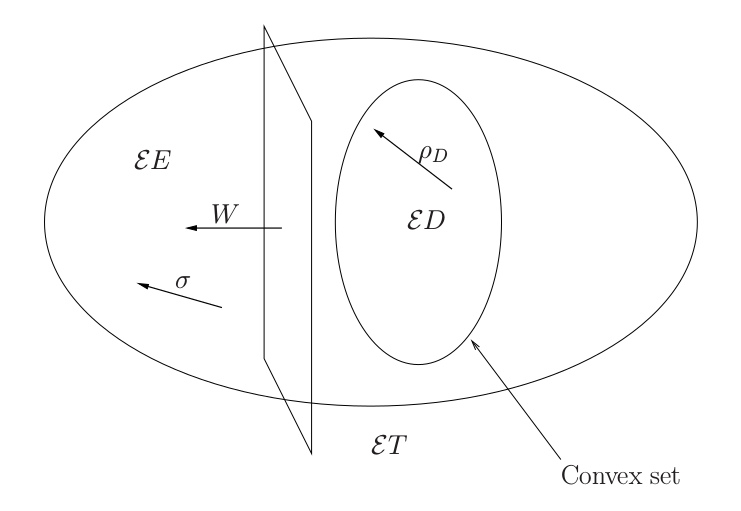
\includegraphics[scale=0.52]{figures/entanglementwitness.png}
    \caption{$D$ is the set of disentangled states and $E$ is the set of entangled states. If there exists a Hermitian operator $W$ which defines a plane between the two sets, then $W$ is called an entanglement witness.\newline Image courtesy of Vlatko Vedral, \textit{Introduction to Quantum Information Science} \cite{vedralqitbook}}
    \label{fig: Entanglement Witnesses}
  \end{center}
\end{figure}
\par To define the witness $W$, first consider an arbitrary vector space $V$. A plane in $V$ is specified by the vectors $\ket{\psi}$ such that
\begin{align*}
\braket{w \mid \psi} = 0
\end{align*}
where $w$ is a unit vector orthogonal to the plane.
\par Hermitian operators can also be thought of as vectors and an inner product can be defined for them as
\begin{align*}
\braket{O_1 \mid O_2} = tr \left( O_1^{\dagger} O_2 \right)
\end{align*}
For a Hermitian operator, that will become
\begin{align*}
\braket{O_1 \mid O_2} = tr \left( O_1 O_2 \right)
\end{align*}
Using this inner product, we can define a plane in the space of Hermitian operators $\tau$,
\begin{align*}
tr ( w \rho ) = 0
\end{align*}
The term on the right side can be a non-zero constant but we choose zero by convention.
\par Now suppose we have an entangled state $\sigma$. Then by our reasoning so far there exists a plane defined by a Hermitian operator $W$ such that $\sigma$ resides on one side and the convex set of all disentangled states resides on the other side. The points on the plane are defined by
\begin{align*}
tr ( \rho W ) = 0
\end{align*}
\par For each disentangled state $\rho_D$ we can either have $tr (\rho_D W) \geq 0$ or $tr (\rho_D W) \leq 0$. We choose $W$ such that $tr (\rho_D W) \geq 0$. Then for all entangled states $\sigma$ on the other side of the plane, $tr (\sigma W) < 0$.
\par Thus our test for entanglement becomes:
\begin{align*}
  tr (\sigma W) < 0 &\rightarrow \sigma \text{ is entangled} \\
  tr (\rho_D W) \geq 0 &\rightarrow \rho_D \text{ is disentangled}
\end{align*}
\par Whenever an entangled state exists an entanglement witness will also exist. Although in practice they can be hard to find. In the case of two qubits, entanglement witnesses are relatively easier to find. As the dimensionality of the system becomes larger, the search becomes harder and harder. \cite{vedralqitbook}

\subsection{The Peres-Horodecki criterion}
The Peres-Horodecki criterion is a reliable test of whether or not a bipartite state is entangled. The test proceeds as follows:
\begin{enumerate}
  \item Take a partial transpose of the density matrix.
  \item If the resultant matrix has a negative eigenvalue, then the state is entangled. Otherwise, the state is separable. (Reminder: A valid density matrix always has eigenvalues $\geq 0$)
\end{enumerate}
\par To calculate the partial transpose of the density matrix, we start by writing the basis states of qubit $A$ as $\ket{i}$ and $\ket{j}$ and the basis states of $B$ as $\ket{k}$ and $\ket{l}$. The density operator of the full system then is
\begin{align*}
\rho = \sum_{ijkl} p_{ijkl} \ket{i} \bra{j} \otimes \ket{k} \bra{l}
\end{align*}
The partial transpose with respect to $B$ will be
\begin{align*}
\left( \ket{k} \bra{l} \right)^T = \ket{l} \bra{k}
\end{align*}
By applying this transformation to the density operator, we get the partial transpose of that density operator.
\begin{align*}
\rho^{T_B} = (I \otimes T) \rho = \sum_{ijkl} p_{ijkl} \ket{i} \bra{j} \otimes \ket{l} \bra{k}
\end{align*}
\par After calculating the eigenvalues of this resultant matrix, if we find a negative eigenvalue then the state is entangled. If all the eigenvalues are zero or positive then the state is separable. \cite{vedralteleportation}

\section{Quantifying Quantum Entanglement}
\par We have seen that there are states that are entangled and states that are disentangled. Now let us go into a little more detail on the subject and ask the question of how to quantify the degree of entanglement contained in a given system. That is, measuring \textquotedblleft how much\textquotedblright\  entanglement is contained within a system. It turns out that we can also concentrate entanglement from a number of partially entangled states to form a smaller number of maximally entangled states.
\par We first specify the \textbf{desirable properties} that any \textquoteleft decent\textquoteright\ measure of entanglement should have. \cite{vedralteleportation}
\begin{enumerate}
  \item For any separable state $\rho$ the measure of entanglement should be zero.
        \begin{align*} E(\rho) = 0 \end{align*}
  \item A local unitary transformation, which is a unitary transformation of the form $U_A \otimes U_B$ and represents a change of basis, should not change the amount of entanglement in a state.
        \begin{align*} E(\rho) = E(U_A \otimes U_B \rho U_A^{\dagger} \otimes U_B^{\dagger}) \end{align*}
  \item Local operations \& classical communication (LOCC) - the act of classically communicating the results of local operations on the subsystems - and sub-selection cannot increase the expected entanglement \cite{vedralteleportation}. If we start with an ensemble in state $\rho$ and end up with sub-ensembles in states $\rho_i$ occurring with probabilities $p_i$, then
        \begin{align*} E(\rho) \geq \sum_i p_i E(\rho_i) \end{align*}
  \item Given two pairs of entangled particles in total state $\rho = \rho_1 \otimes \rho_2$, their entanglement is additive.
        \begin{align*} E(\rho) = E(\rho_1) + E(\rho_2) \end{align*}
\end{enumerate}
\par Now we shall look at some actual measures of entanglement which fulfill these requirements to be \textquoteleft decent\textquoteright\  entanglement measures. \cite{plenioentanglementmeasures}

\subsection{Entropy of Entanglement}
\par The entropy of entanglement is, in simple terms, the von Neumann entropy of the reduced density matrix of the given pure state.
\begin{align*}
S(\rho_A) = - tr \{ \rho_A \log \rho_A \}
\end{align*}
where $\rho_A$ is the reduced density matrix for subsystem $A$, obtained by tracing out subsystem $B$. That is, $\rho_A = tr_B \{\rho_{AB}\}$.
\par Entropy of entanglement suffers from the limitation that it only works as a good measure of entanglement for pure states. It does not work when mixed states are involved.

\subsection{Linear Entropy of Entanglement}
\par Linear entropy of entanglement is a linear approximation to the entropy of entanglement, in the same way that linear entropy is the linear approximation to von Neumann entropy. It is easier to calculate than the entropy of entanglement. The basic idea is the same: tracing out subsystem $B$ to obtain the reduced density matrix for subsystem $A$ and then taking its linear entropy.
\begin{align*}
S_L(\rho_A) = 1 - tr(\rho_A^2)
\end{align*}
\par This measure also suffers from the same problem as the entropy of entanglement. It does not work for mixed states. It can only work as a decent entanglement measure for pure states.

\subsection{Renyi Entanglement Entropy}
Renyi entanglement entropy of a density matrix $\rho$ is also defined in terms of its reduce density matrix $\rho_A$ or $\rho_B$.
\begin{align*}
S_\alpha (\rho_A) &= \frac{1}{1-\alpha} \log (tr\{\rho_A^\alpha\}) , \quad \alpha \neq 1 \: \text{and} \: \alpha > 0
\end{align*}
In terms of the eigenvalues of the reduced density matrix $q_i$,
\begin{align*}
S_\alpha (\rho_A) &= \frac{1}{1-\alpha} \log \left( \sum_i q_i^\alpha \right)
\end{align*}
where $\alpha$ is the Renyi index.
\par In the limit $\alpha \rightarrow 1$ it approaches the von Neumann entropy.

\subsection{Negativity}
\par Peres-Horodecki criterion tests for entanglement by presence of negative eigenvalues under partial transpose. Negativity is a measure of how negative the resulting matrix is. Mathematically, it is defined as
\begin{align*}
N(\rho) = \frac{\lVert \rho^{T_A} \rVert_1 - 1}{2}
\end{align*}
where $\rho^{T_A}$ is the partial transpose of the density matrix with respect to $A$ and $\lVert . \rVert_1$ denotes the trace norm.
\par Negativity has the property of non-increase under LOCC. But it does not have the additivity property. This brings us to logarithmic negativity.

\subsection{Logarithmic Negativity}
\par The logarithmic negativity of a bipartite state is
\begin{align*}
E_N(\rho) = log_2 \lVert \rho^{T_A} \rVert_1
\end{align*}
\par Logarithmic negativity is additive and provides an upper bound on how much entanglement can be distilled from a system.

\subsection{Concurrence}
\par Concurrence of a bipartite state $\rho$ is defined as
\begin{align*}
C(\rho) = max(0, \lambda_1 - \lambda_2 - \lambda_3 - \lambda_4)
\end{align*}
i.e. the greater one of these two quantities. The numbers $\lambda_1 > \lambda_2 > \lambda_3 > \lambda_4$ are eigenvalues of the Hermitian matrix
\begin{align*}
R = \sqrt{ \sqrt{\rho} \tilde{\rho} \sqrt{\rho} }
\end{align*}
in which
\begin{align*}
\tilde{\rho} = ( \sigma_y \otimes \sigma_y ) \rho^* ( \sigma_y \otimes \sigma_y )
\end{align*}
where $\rho^*$ is the complex conjugate of $\rho$ and $\sigma_y$ is the Pauli spin matrix known by the same label.
\par The value of concurrence ranges from 0 to 1. It is 0 for separable states and 1 for the maximally entangled state.
\par For multipartite states, concurrence takes on a more complicated form than the one shown here.

\subsection{Relative Entropy of Entanglement}
\par The basic idea for relative entropy of entanglement is based on distinguishability and geometrical distance. In this approach, when given a state $\sigma$, we compare its distance to each state from the whole set of disentangled states $D$ and pick the state $\rho$ which has the minimum distance from $\sigma$. The relative entropy of entanglement is thus this minimum distance.

\begin{align*}
E_{RE}(\sigma) = \underset{\rho \in D}{\min}  D(\sigma||\rho)
\end{align*}

\begin{figure}[h]
  \begin{center}
    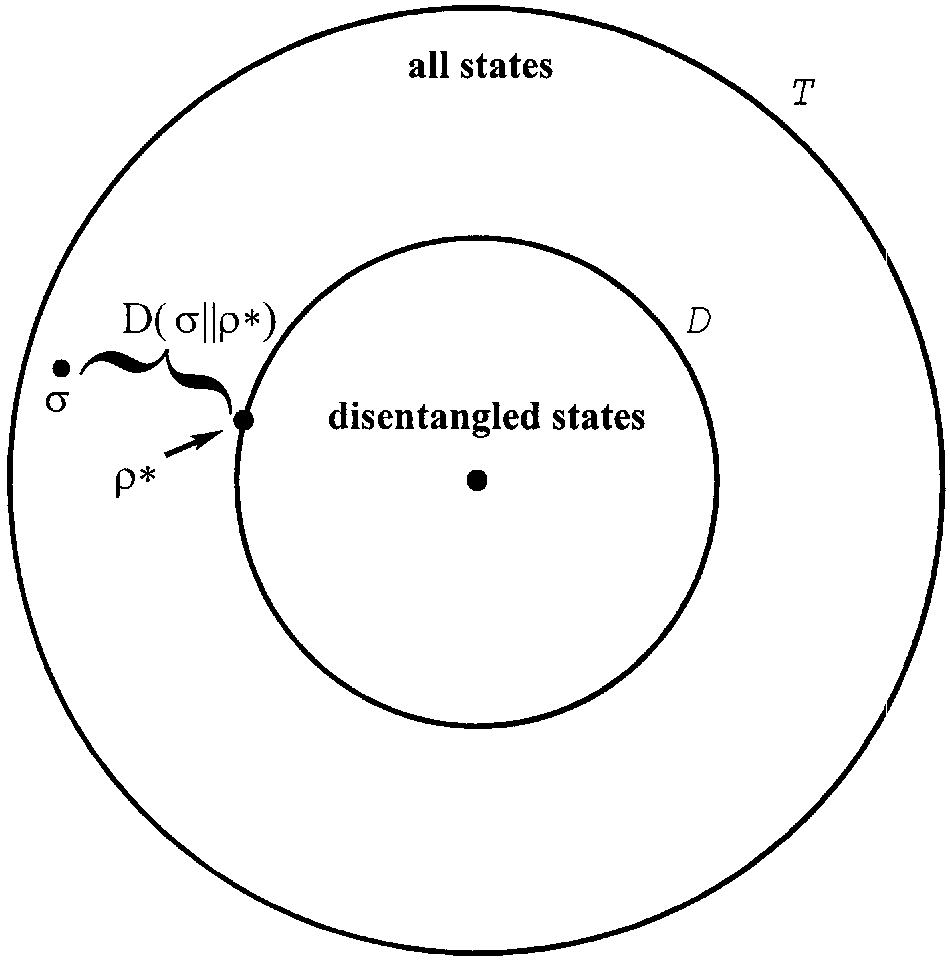
\includegraphics[scale=0.25]{figures/entanglement-distance.png}
    \caption{Relative entropy of entanglement: the distance from the nearest disentangled state\newline $\sigma$ is the state for which the quantity is to be measured. Over the whole state of disentangled states $\{\rho\}$, the state $\rho^*$ has the minimum distance from $\sigma$. The distance to $\rho^*$ is the relative entropy of entanglement of $\sigma$.\newline Image courtesy of Vlatko Vedral, \textit{Introduction to Quantum Information Science} \cite{vedralqitbook}}
    \label{fig: Relative Entropy of Entanglement}
  \end{center}
\end{figure}

\par Here the function $D$ is a measure of separation between the two density matrices. There are a number of separation measures available to define the \textquoteleft distance\textquoteright \  between two density matrices. Though it should be noted that not all distance measures will generate a \textquoteleft decent\textquoteright \  entanglement measure by our criteria. Those requirements have to be kept in mind when looking for an entanglement measure.

\par One distance measure which generates an entanglement measure satisfying the \textquoteleft decency\textquoteright \  criteria is the Kullback-Leibler distance - alternatively known as the relative entropy - that we talked about in section 3.5.2.
\begin{align*}
S(\sigma||\rho) &= tr \{ \sigma \log \sigma - \sigma \log \rho \}
\end{align*}
\par We can plug this into the formula for relative entropy of entanglement to generate an entanglement measure. We can similarly use many other distance measures in place of the Kullback-Leibler distance.
\par Relative entropy of entanglement is an important quantity because we can plug in various distance measures in place of the distance function $D$ and so we can derive many other entanglement measures from it - provided that they satisfy the criteria for decent entanglement measures. \cite{vedralteleportation}


\chapter{Computational Tools in Quantum Information Theory}
\chaptermark{Computational Tools in QIT}

\par Traditionally physics research has been divided into "theoretical" and "experimental" physics: theoretical physics focusing on a rigorous mathematical framework for understanding our world and experimental physics concerned with testing the validity of the theories in a laboratory. With the increasing penetration of computers in how we do our work, the way we do physics research has inevitably experienced some changes. In recent years there has been a growing body of work in "computational physics" which is concerned with doing numerical experiments in a computer laboratory looking at how different theories should play out. This provides an intersection between theoretical and experimental physics where theories are analyzed numerically and the results are then compared to real world data from a laboratory. This has a great contribution in accelerating physics research. Some people call this approach "experimental mathematics". \cite{wolframexperimentalmath}
\par This chapter discusses some of the tools available to apply the techniques of computational physics to quantum information theory. As the situation is, physicists do not normally have the luxury of canned computer programs readily available for their work so they have to write the programs themselves. The "tools" talked about here are simply: programming languages and libraries/toolboxes to facilitate writing programs for a particular kind of problem.
\par Looking at the available programming languages we encounter many that we can potentially use to solve physics problems. There are C, C++, FORTRAN, Java, Python, MATLAB and Lisp just to name a few. Each of these has its own strengths and use cases where it excels. C and C++, for example, generate extremely fast compiled native code. Java programs, written once, can run on virtually any hardware. FORTRAN has a large body of legacy physics code. This project looks at two of these languages: MATLAB and Python.

\section{MATLAB}
MATLAB, which stands for MATrix LABoratory, is a self-contained proprietary programming environment developed by MathWorks to help scientists and engineers write numerical programming applications. As its name implies, it bases itself on matrices. It is a commercial product. By a self-contained environment we mean that it is a single package consisting of an integrated development environment tightly integrated with its own programming language and collection of libraries - or toolboxes as they are called. In this text when we refer to MATLAB, we will mostly mean the programming language.
\par MATLAB is a high level programming language designed for a special domain - i.e. scientific and engineering applications. In that it does a pretty good job. With its high level of abstractions it removes all the unnecessary worries of the underlying hardware. It has built in tools for plotting and simulations. It has a large collection of toolboxes pre-packaged for a variety of tasks ranging from solving differential equations to symbolic computing and digital signal processing. Additional toolboxes are also available which can be easily added and used. It also provides tools for designing basic graphical user interfaces for when the need arises.
\par Before we move on to the topic of quantum information toolboxes in MATLAB, we shall go through a basic tutorial of MATLAB to give the reader a feel of how it works. It is assumed that the user has a prior basic knowledge of working with any other programming language.

\subsection*{Tutorial: MATLAB Basics}
In this tutorial we shall be entering some basic commands at the MATLAB interactive prompt. \texttt{>>} is the MATLAB prompt and indicates that MATLAB is ready to accept an input command or statement. What shows up after entering the command is the output.
\par We start with variables. In MATLAB, variables are dynamically typed. That is, the type of the variable does not have to be declared before storing the value. Variables are also case sensitive.
\begin{verbatim}
>> a = 5
a = 
    5
>> b = 7
b = 
    7
>> B = 3
B = 
    3
>> a+b+B
ans = 
    15
\end{verbatim}
The basic data structure, of course, is a matrix. In fact the earlier examples are special cases of 1x1 matrices. Now let us use some vectors.
\begin{verbatim}
>> c = [1,5,3]
c =
   1   5   3

>> d = [4;3;7]
d =
   4
   3
   7

>> c*d
ans = 
      40

>> d*c
ans =
    4   20   12
    3   15    9
    7   35   21
\end{verbatim}
We can also select a particular element using indices.
\begin{verbatim}
>> d(1)
ans = 
      4
      
>> (d*c)(2,2)
ans = 
     15   
\end{verbatim}
We end our tutorial with a simple for loop.
\begin{verbatim}
>> for i=1:3
    disp(i)
   end

 1
 2
 3
\end{verbatim}
The more curious reader can consult one of the many detailed books on MATLAB. \cite{allendowneymatlab}

\subsection*{QI Toolboxes for MATLAB}
\par Due to MATLAB's popularity in academia over the years, a lot of research code has been written in MATLAB and a lot of people have written toolboxes for applications in science and engineering. This gives it a huge advantage as a programming language. For someone to understand and build upon such a previous work, learning MATLAB is a pre-requisite. A whole body of previous work is what keeps MATLAB relevant today.
\par Toolboxes have been written for quantum information work too. The following MATLAB toolboxes were explored as part of this project.

\subsection{QLib}
QLib is a free and open source toolbox written for quantum information research by Shai Machnes at the Tel-Aviv University \cite{qlib}. It provides a rich collection of functions to implement the ideas of QIT and explore questions with help from its visualization tools and optimization algorithms. Its features include simulating of quantum states including entangled states, various measures of entropy and entanglement, functions for measurements, Schmidt decomposition, gates, distance measures between density matrices, plotting and many more.
\par Let us take a look at some example code. This basic example parametrizes a random pure state and then performs the partial transpose entanglement test on it.
\begin{verbatim}
>> pure = param_pure_1_rand([2 2])
pure =
   0.4839 + 0.0000i
  -0.4078 + 0.0046i
   0.4005 - 0.3689i
  -0.5500 - 0.0236i

>> is_entangled_pt(pure)
ans =
     1
\end{verbatim}
\par This example plots the negativity vs concurrence of 10,000 random density matrices of two qubits.
\begin{verbatim}
neg = []; con = [];
for k=1:10000
    dm = param_dm_2x_rand([2 2]);
    neg(k) = negativity(dm);
    con(k) = concurrence(dm);
end
scatter(neg,con,2);
\end{verbatim}
The result is this plot.
\begin{figure}[H]
  %\begin{center}
    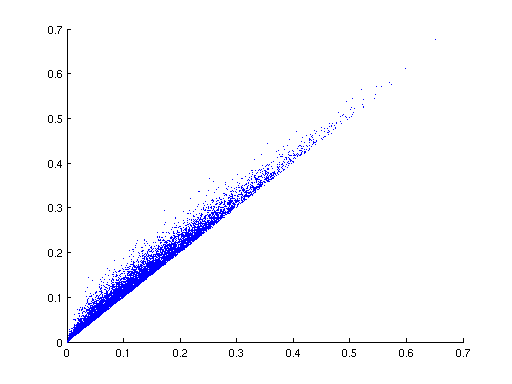
\includegraphics[scale=0.88]{figures/qlib-negativity-vs-concurrence.png}
    \caption{QLib: Negativity vs Concurrence of 10,000 random DMs.\newline X-axis: Negativity, Y-axis: Concurrence}
    \label{fig: QLib: Negativity vs Concurrence}
  %\end{center}
\end{figure}

\subsection{QETLAB}
QETLAB (Quantum Entanglement Theory LABoratory) is another free and open source toolbox for quantum information work. It was started and is primarily maintained by Nathaniel Johnston at the Mount Allison University, Canada \cite{qetlab}. As its name implies, it specifically aims to provide functionality related to entanglement. The goal of the project is to remain up to date with an ever-growing catalogue of separability criteria, positive maps, and related functions of interest. Compared to QLib, this toolbox is more recent and is under active maintenance at the time of this writing.
\par Let us look at some example code. This example generates a random 2x2 density matrix and calculates its von Neumann entropy.
\begin{verbatim}
>> rho = RandomDensityMatrix(2)
rho =
   0.83755 + 0.00000i  -0.01727 - 0.00114i
  -0.01727 + 0.00114i   0.16245 + 0.00000i

>> Entropy(rho)
ans =  0.63909
\end{verbatim}

This example generates a random state vector and then calculates its Schmidt decomposition.
\begin{verbatim}
>> d = 2
d =  2
>> phi = RandomStateVector(d^2)
phi =
   0.35227 + 0.32456i
  -0.37642 + 0.23467i
  -0.22955 - 0.66080i
   0.17927 - 0.22872i

>> [s,u,v] = SchmidtDecomposition(phi)
s =
   0.96858
   0.24872

u =
  -0.64481 + 0.00000i   0.76434 - 0.00000i
   0.73711 + 0.20221i   0.62184 + 0.17058i

v =
  -0.547168 - 0.671034i   0.055448 - 0.497238i
   0.339278 - 0.367710i  -0.865439 + 0.026381i

\end{verbatim}
The entries of \texttt{s} are the Schmidt coefficients and the columns of \texttt{u} and \texttt{v} are the left and right Schmidt vectors respectively.

\subsection{Quantum Information Toolkit}
Quantum Information Toolkit is an open source quantum information toolbox available for both MATLAB and Python developed by Ville Bergholm et al. \cite{quantuminformationtoolkit}. Its MATLAB and Python versions both contain equivalent functionality. We shall discuss it in detail in the Python section.

\pagebreak

\section{Python}
Python \cite{python} \cite{primerscientificpython} is a free and open source, multi-paradigm, general purpose programming language. By multi-paradigm we mean that it can be used to code in the procedural, object oriented or functional programming styles. It is cross-platform and can run from desktops and servers to mobile devices and even small embedded systems like network routers or miniature computers like the Raspberry Pi. This gives it the flexibility to be used in pretty much any environment for almost any purpose. We find it being used in desktop and server applications, industrial automation, robotics, scientific research and control systems. In scientific research it can be used for mathematical modeling, simulation, laboratory automation, signal processing, data analysis and numerous other tasks.
\par Python's design philosophy makes it very easy to learn the language and also makes it easy to read and understand other people's code. Furthermore, its high level abstractions make it an ideal language for rapid prototyping. This makes it an attractive language to implement scientific ideas in. Hence over the years, it has accumulated a vast collection of libraries to do many kinds of scientific computations. In addition to that, it also has a large collection of libraries to help with many other kinds of programming. Hence the researchers who learn Python also have access to a lifetime supply of tools to implement their ideas in any way they like: be it providing a web interface to their signal processing tool, writing a good looking graphical interface to present their research, plotting their data in a variety of forms or explaining their code step by step in an iPython notebook. They have numerous options to make their research more immediately useful to the community. This makes Python an increasingly popular programming language within the scientific community.
\par Before we proceed to discuss the quantum information toolboxes available for Python, we should briefly mention the popular libraries NumPy, SciPy and SymPy which have become ubiquitous among the scientific programming community. Many of the other scientific libraries build on top of these.

\subsection{NumPy}
Numpy \cite{numpy} adds support for large multi-dimensional arrays and matrices to Python. It also provides a large library of mathematical functions to operate on those arrays. It is the go-to library for Python when dealing with large scale number-crunching and contains very powerful mathematical functions. NumPy is free and open source software and many other numerical solutions for Python build on top of NumPy.
\par Let us look at a simple example of solving some basic linear algebra problems.
\begin{verbatim}
>>> import numpy as np
>>> from numpy.linalg import solve, inv
>>> a = np.matrix([[2.4,3.5,1.3],[6.2,7.1,3.9],[5.5,9.0,8.4]])
>>> a.transpose()
matrix([[ 2.4,  6.2,  5.5],
        [ 3.5,  7.1,  9. ],
        [ 1.3,  3.9,  8.4]])
>>> inv(a)
matrix([[-0.92485113,  0.66706867, -0.16657873],
        [ 1.15436798, -0.49031431,  0.04899374],
        [-0.63126555,  0.08856561,  0.17562373]])
>>> b =  np.array([3, 4, 5])
>>> solve(a, b)    # solve for equation ax = b
array([-0.93917238,  1.74681541, -0.66141554])
\end{verbatim}

\subsection{SciPy}
SciPy \cite{scipy} is a more general scientific programming library for Python. It builds on top of NumPy and adds its own huge library of modules and functions for many tasks common in science and engineering. Some of these tasks are optimization, linear algebra, integration, interpolation, special functions, fast Fourier transform, signal and image processing and ordinary differential equation solvers. Like NumPy, SciPy is also free and open source software.

\subsection{SymPy}
SymPy \cite{sympy} is a Python module for symbolic computations, unlike NumPy discussed earlier which is built for numerical computations. By symbolic computations, we mean computations of mathematical objects symbolically: the mathematical objects are represented exactly, not approximately, and mathematical expressions with unevaluated variables are left in symbolic form.
\par Let us look at an example of a basic integral.
\begin{verbatim}
>>> from sympy import *
>>> x = symbols('x')
>>> integrate(exp(x)*sin(x) + exp(x)*cos(x), x)
exp(x)*sin(x)
\end{verbatim}
We see that rather than requiring or computing the numerical value for $x$, it is treated in symbolic form.
\par Just like NumPy and SciPy, SymPy is also free and open source.

\subsection{matplotlib}
matplotlib \cite{matplotlib} is an open source plotting library for Python. It is normally used with NumPy to produce high quality plots of mathematical functions and scientific data. SciPy also makes use of it. matplotlib's pyplot interface provides an interface very similar to MATLAB's plotting.
\par Let us look at a basic plotting example.
\begin{verbatim}
>>> import numpy as np
>>> import matplotlib.pyplot as plt
>>> x = np.linspace(0, 1, 100)
>>> y = np.sin(4 * np.pi * x) * np.exp(-5 * x)
>>> plt.plot(x, y)
>>> plt.grid(True)
>>> plt.show()
\end{verbatim}
This results in the following plot.
\begin{figure}[H]
  \begin{center}
    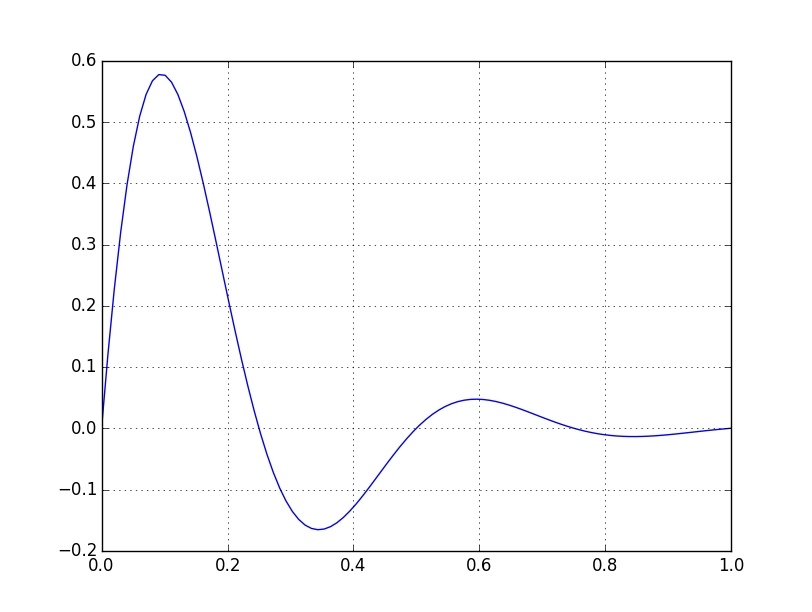
\includegraphics[scale=0.55]{figures/matplotlibexample.png}
    \caption{Plotting with matplotlib}
    \label{fig: matplotlib Example}
  \end{center}
\end{figure}

\par Now that we have become familiar with the more essential and more popular scientific modules in the Python ecosystem, we shall proceed to discuss the ones specific to quantum information theory.

\subsection{qitensor}
qitensor is a quantum information module for Python written by Dan Stahlke \cite{qitensor}. It is based on NumPy and adds functionality to facilitate working with finite dimensional quantum mechanics of many particles. It also has preliminary support for symbolic calculations through SymPy.
\par A simple example using qitensor:
\begin{verbatim}
>>> from qitensor import qubit
>>> ha = qubit('a')
>>> hb = qubit('b')
>>> ha * hb
|a,b>
>>> x = (ha * hb).array()
>>> x
HilbertArray(|a,b>,
array([[ 0.+0.j,  0.+0.j],
       [ 0.+0.j,  0.+0.j]]))
\end{verbatim}

\subsection{Quantum Information Toolkit}
Quantum Information Toolkit, developed by Ville Bergholm et al. \cite{quantuminformationtoolkit}, is a free and open source quantum information toolbox for both MATLAB and Python. The MATLAB and Python versions both contain equivalent functionality. The Python version builds upon the NumPy, SciPy and matplotlib libraries.
\par Some example code from the Python version:
\begin{verbatim}
>>> a = state('0')
>>> b = state('1')
>>> a.measure()
(array([ 1.,  0.]), 0)
>>> b.measure()
(array([ 0.,  1.]), 1)
>>> a * b.transpose() 
array([[ 0.,  1.],
       [ 0.,  0.]])
dim: (2,) <- (2,)
>>> ab = tensor(a,b)
>>> ab.data
array([[ 0.],
       [ 1.],
       [ 0.],
       [ 0.]])
\end{verbatim}

\subsection{Quantum Toolbox in Python (QuTiP)}
QuTiP \cite{qutipdoc} is a very large free and open source toolbox for simulating open quantum systems. Started by Robert J. Johansson of RIKEN Japan and Paul D. Nation of Korea University, it has grown into a large collaborative project involving researchers from many other institutes. Like many toolboxes previously discussed, it also builds on top of NumPy and SciPy and uses matplotlib for plotting. It also optimizes for speed by using Cython to make Python code many times faster and by parallelizing tasks when possible.
\par Unlike the other toolboxes discussed so far, this one is not specific to quantum information. However it does have a great internal structure and a huge library of functions to simulate a wide variety of quantum systems. The efficiency in terms of computation time is also very good. On top of that, it is actively maintained, widely used and has a larger community to get help from. This makes it a good choice as a toolbox to implement quantum information functions in.
\par Extending QuTiP with quantum information functionality is the main theme of this project. Hence the whole next chapter is dedicated to it. The next chapter starts with the basics of how QuTiP works and how more functions can be written on top of it. Then it demonstrates the code written for this project, including the addition of QI functions to QuTiP and making use of them in simulations.
\par For now, we can use a simple example as an introduction, dealing with these two states.
\begin{align*}
\ket{\psi_0} &= \ket{\uparrow} \\
\ket{\psi_1} &= \frac{1}{\sqrt{2}} \left( \ket{\uparrow} + \ket{\downarrow} \right)
\end{align*}

\begin{verbatim}
>>> from qutip import *
>>> import numpy as np
>>> up = basis(2,0)
>>> dn = basis(2,1)
>>> psi0 = up
>>> psi1 = 1/np.sqrt(2) * ( up + dn )
>>> print(psi0)
Quantum object: dims = [[2], [1]], shape = [2, 1], type = ket
Qobj data =
[[ 1.]
 [ 0.]]
>>> print(psi1)
Quantum object: dims = [[2], [1]], shape = [2, 1], type = ket
Qobj data =
[[ 0.70710678]
 [ 0.70710678]]
>>> # The density matrix for an equal mixture of both states
>>> rho = 0.5 * ( ket2dm(psi0) + ket2dm(psi1) )
>>> print(rho)
Quantum object: dims = [[2], [2]], shape = [2, 2], type = oper, isherm = True
Qobj data =
[[ 0.75  0.25]
 [ 0.25  0.25]]
\end{verbatim}


\chapter{Getting Started with QuTiP}

\par This chapter discusses the basics of QuTiP and how it can be used in quantum information work.

\section{QuTiP Basics}
QuTiP is a large library. Understanding all of it will need much more background knowledge than the scope of this project. Here we only explain some basics to help the reader get started. The more curious reader can consult the QuTiP documentation. \cite{qutipdoc}
\par First of all we need to understand the basic data structure which represents quantum states, operators and other matrices in QuTiP. This is called the quantum object class (\texttt{Qobj}) in QuTiP.

\subsection{The Quantum Object Class}
The quantum object, or \texttt{Qobj} in short, is the basic data structure that all of QuTiP's functions will work on. It is a matrix with some context information added about what exactly it represents in terms of quantum mechanics. In addition to the data about what it represents, it also has various built-in methods to perform calculations on it.
\par To get started, let us create a simple blank \texttt{Qobj}. The qutip module will need to be imported first. Most of our code will also use functions from NumPy so we import that too.
\begin{verbatim}
In [1]: from qutip import *
In [2]: import numpy as np
\end{verbatim}
This imports all functions from the qutip module and imports numpy with a shorter name np for convenience. Now we are ready to create a Qobj instance.
\begin{verbatim}
In [3]: Qobj()
Out[3]:
Quantum object: dims = [[1], [1]], shape = [1, 1], type = oper, isherm = True
Qobj data =
[[ 0.]]
\end{verbatim}
We see that calling Qobj() without any arguments returns a 1x1 matrix with a zero entry. There is also some additional information printed out: the dimensions of the object, its type which is an operator and whether or not the matrix is Hermitian. There is also additional information stored in the Qobj which is not displayed here or in a simple print statement.
\par The Qobj can also take user input, for example, for the entries of the matrix.
\begin{verbatim}
In [4]: Qobj([[1],[0]])
Out[4]: 
Quantum object: dims = [[2], [1]], shape = [2, 1], type = ket
Qobj data =
[[ 1.]
 [ 0.]]
In [5]: Qobj([[1,0],[0,0]])
Out[5]: 
Quantum object: dims = [[2], [2]], shape = [2, 2], type = oper, isherm = True
Qobj data =
[[ 1.  0.]
 [ 0.  0.]]
\end{verbatim}
In the above example, we used a list of lists as input. We could also have used a numpy array or matrix. For more information on how to initialize a Qobj instance, the reader can use the built-in help: \texttt{help(Qobj)}

\subsection{Basic Operations on Quantum Objects}
Let us try to create this state in QuTiP.
\begin{align*}
\ket{\psi_1} = \frac{2}{\sqrt{5}} \ket{0} + \frac{1}{\sqrt{5}} \ket{1}
\end{align*}

\begin{verbatim}
In [1]: from qutip import *
In [2]: import numpy as np
In [3]: up = basis(2,0)
In [4]: dn = basis(2,1)
In [5]: print(up)
Quantum object: dims = [[2], [1]], shape = [2, 1], type = ket
Qobj data =
[[ 1.]
 [ 0.]]
In [6]: psi1 = ( 2/np.sqrt(5) * up ) + ( 1/np.sqrt(5) * dn )
In [7]: print(psi1)
Quantum object: dims = [[2], [1]], shape = [2, 1], type = ket
Qobj data =
[[ 0.89442719]
 [ 0.4472136 ]]
\end{verbatim}
The function \texttt{basis(2,0)} creates a state ket vector of length 2 with its zeroth index (i.e. first entry) as 1 and the rest of the entries zero. Similarly \texttt{basis(2,1)} makes the second entry 1 and the rest zero.
\par To calculate the density matrix for $\ket{\psi_1}$, we can multiply it with its conjugate transpose ( \texttt{psi1.dag()} ) or simply use the function \texttt{ket2dm} provided by QuTiP which takes a ket vector and returns its density matrix.
\begin{verbatim}
In [8]: psi1 * psi1.dag()
Out[8]: 
Quantum object: dims = [[2], [2]], shape = [2, 2], type = oper, isherm = True
Qobj data =
[[ 0.8  0.4]
 [ 0.4  0.2]]
 
In [9]: ket2dm(psi1)
Out[9]: 
Quantum object: dims = [[2], [2]], shape = [2, 2], type = oper, isherm = True
Qobj data =
[[ 0.8  0.4]
 [ 0.4  0.2]]
\end{verbatim}
For tensor products, QuTiP has a built-in function \texttt{tensor}.
\begin{verbatim}
In [10]: tensor(up,dn)
Out[10]: 
Quantum object: dims = [[2, 2], [1, 1]], shape = [4, 1], type = ket
Qobj data =
[[ 0.]
 [ 1.]
 [ 0.]
 [ 0.]]
\end{verbatim}
Notice how the dimensions value changes because now we are representing a composite object in an extended Hilbert space.
\par Let us now create a maximally entangled state
\begin{align*}
\ket{\psi_{AB}} = \frac{1}{\sqrt{2}} \left( \ket{0}_A \ket{0}_B + \ket{1}_A \ket{1}_B \right)
\end{align*}

\begin{verbatim}
In [11]: psi_ab = 1/np.sqrt(2) * ( tensor(up,up) + tensor(dn,dn) )

In [12]: print(psi_ab)
Quantum object: dims = [[2, 2], [1, 1]], shape = [4, 1], type = ket
Qobj data =
[[ 0.70710678]
 [ 0.        ]
 [ 0.        ]
 [ 0.70710678]]
\end{verbatim}
\par QuTiP also has a shortcut to create maximally entangled states (also known as Bell states) via the \texttt{bell\_state} function.
\begin{verbatim}
In [13]: bell_state('00')
Out[13]: 
Quantum object: dims = [[2, 2], [1, 1]], shape = [4, 1], type = ket
Qobj data =
[[ 0.70710678]
 [ 0.        ]
 [ 0.        ]
 [ 0.70710678]]
\end{verbatim}
The input argument to \texttt{bell\_state} is one of '00', '01', '10' or '11' representing the four Bell states.
\par Let us now calculate some properties of \texttt{psi\_ab}.
\begin{verbatim}
In [16]: entropy_vn(psi_ab)
Out[16]: 2.220446049250313e-16

In [17]: concurrence(psi_ab)
Out[17]: 0.99999999999999978
\end{verbatim}
We can see that its von Neumann entropy is 0 within computational error range and concurrence is 1, as expected.
\par To take the trace of the density matrix for $\ket{\psi_{AB}}$, we use the \texttt{tr()} method for the \texttt{Qobj}. We can see that the trace values for the density matrix and the density matrix squared are 1, indicating a pure state as expected.
\begin{verbatim}
In [20]: ket2dm(psi_ab).tr()
Out[20]: 0.9999999999999998

In [21]: (ket2dm(psi_ab)**2).tr()
Out[21]: 0.9999999999999996
\end{verbatim}
\par QuTiP also has a partial trace operation which shall be useful in our calculations.
\begin{verbatim}
In [22]: ptrace(psi_ab,0)
Out[22]: 
Quantum object: dims = [[2], [2]], shape = [2, 2], type = oper, isherm = True
Qobj data =
[[ 0.5  0. ]
 [ 0.   0.5]]
\end{verbatim}
The \texttt{ptrace} function accepts state vectors as well as density matrices as input. The second argument is which subsystems to keep in the partial trace. In this case, 0 is for A and 1 is for B. We have told it to calculate the density matrix for subsystem A.
\par Let us now calculate the probability of projecting atom A on ground state ($\ket{0}$ or $\ket{\uparrow}$) and B on excited state ($\ket{1}$ or $\ket{\downarrow}$). First we shall need to calculate the projector $\ket{0} \bra{0} \otimes \ket{1} \bra{1}$. Then we apply it to the density matrix and take the trace to find the probability of the atoms collapsing to that state.
\begin{verbatim}
In [24]: a0 = up * up.dag()
In [25]: b1 = dn * dn.dag()
In [26]: prj_a0b1 = tensor(a0,b1)
In [27]: print(prj_a0b1)
Quantum object: dims = [[2, 2], [2, 2]], shape = [4, 4], type = oper, 
isherm = True
Qobj data =
[[ 0.  0.  0.  0.]
 [ 0.  1.  0.  0.]
 [ 0.  0.  0.  0.]
 [ 0.  0.  0.  0.]]
In [28]: print(ket2dm(psi_ab))
Quantum object: dims = [[2, 2], [2, 2]], shape = [4, 4], type = oper, 
isherm = True
Qobj data =
[[ 0.5  0.   0.   0.5]
 [ 0.   0.   0.   0. ]
 [ 0.   0.   0.   0. ]
 [ 0.5  0.   0.   0.5]]
In [29]: res_matrix = prj_a0b1 * ket2dm(psi_ab)
In [30]: print(res_matrix)
Quantum object: dims = [[2, 2], [2, 2]], shape = [4, 4], type = oper, 
isherm = True
Qobj data =
[[ 0.  0.  0.  0.]
 [ 0.  0.  0.  0.]
 [ 0.  0.  0.  0.]
 [ 0.  0.  0.  0.]]
In [31]: res_matrix.tr()
Out[31]: 0.0
\end{verbatim}
\par The expectation value is \textit{zero} which means that if we measure the states of the atoms, there is no chance that we will find them anticorrelated such that the atom A is in ground state and the atom B is in excited state. This is in agreement with what we would expect by simply looking at the equation of the entangled state where the coefficient for $\ket{0}_A \ket{1}_B$ is zero.
\par QuTiP provides an easier way to calculate the expectation values of operators on states via the \texttt{expect} function.
\begin{verbatim}
In [36]: expect(prj_a0b1,psi_ab)
Out[36]: 0.0
In [37]: expect(prj_a0b1,ket2dm(psi_ab))
Out[37]: 0.0
\end{verbatim}
The \texttt{expect} function takes an operator and one or more states. For states, we can pass it the ket vector or the density matrix.

\section{Quantum Information Computations with QuTiP}
Now that we have demonstrated the basics of QuTiP, we move on to some slightly advanced calculations involving quantum information. All of the calculations and simulations appearing next have been based on Plenio's review paper \cite{pleniophysforget}.
\subsection{No Cloning of Quantum Bits}
The no-cloning theorem in quantum information theory states that quantum bits cannot be cloned \cite{nielsenchuang}. In this part, with the help of a practical example, we make an argument for its validity. We start with a thought experiment where Alice sends Bob a message encoded in quantum states and Bob has to extract that information. We take a look at what would happen if Bob could clone those quantum bits that he receives.
\par Initially Alice encodes symbols 0 and 1, occurring with equal probabilities, in the non-orthogonal states $\ket{\psi_0}$ and $\ket{\psi_1}$.
\begin{align*}
0 \longmapsto \ket{\psi_0} &= \ket{\uparrow} \\
1 \longmapsto \ket{\psi_1} &= \frac{1}{\sqrt{2}} \ket{\uparrow} + \frac{1}{\sqrt{2}} \ket{\downarrow}
\end{align*}

\begin{verbatim}
In [1]: from qutip import *
In [2]: import numpy as np
In [3]: up = basis(2,0)
In [4]: dn = basis(2,1)
In [5]: psi0 = up
In [6]: psi1 = 1/np.sqrt(2) * ( up + dn )
\end{verbatim}

The upper bound to information transmitted per letter is given by $S(\rho)$ where $\rho$ represents the incomplete knowledge that we have of the state of each carrier.
\begin{align*}
\rho = \frac{1}{2} \ket{\psi_0} \bra{\psi_0} + \frac{1}{2} \ket{\psi_1} \bra{\psi_1}
\end{align*}

\begin{verbatim}
In [7]: rho = 0.5 * ( ket2dm(psi0) + ket2dm(psi1) )
In [8]: entropy_vn(rho,2)
Out[8]: 0.6008760366928562
\end{verbatim}
The second argument for \texttt{entropy\_vn} is the base of log used when calculating the von Neumann entropy, which is 2 here since there are two possible states. Notice that the von Neumann entropy is less than 1 bit due to non-orthogonality of the states.
\par Now Alice transmits her message, encoded in these symbols, to Bob who knows the encoding procedure for the symbols but does not know the exact message. The maximum information that Bob can recover is the information that Alice has encoded: i.e. $S(\rho) = 0.6008760366928562$
\par Now let us assume that Bob can somehow clone an arbitrary unknown quantum state. If that happens then upon receiving $\ket{\psi_0}$ or $\ket{\psi_1}$ he can create a copy. In such a situation he will end up with two copies of the 0 state $\ket{\psi_0} \ket{\psi_0}$ and two copies of the 1 state $\ket{\psi_1} \ket{\psi_1}$ which will both occur with equal probability 0.5. The density operator for this situation will be
\begin{align*}
\rho_{2copies} = \frac{1}{2} \ket{\psi_0} \ket{\psi_0} \bra{\psi_0} \bra{\psi_0} + \frac{1}{2} \ket{\psi_1} \ket{\psi_1} \bra{\psi_1} \bra{\psi_1}
\end{align*}
Let us now calculate how much information Bob can recover from this state after he has cloned the qubits. That will be the von Neumann entropy of this new state, $S(\rho_{2copies})$.
\begin{verbatim}
In [10]: psi0psi0 = tensor(psi0,psi0)
In [11]: psi1psi1 = tensor(psi1,psi1)
In [12]: rho_2cp = 0.5 * ( ket2dm(psi0psi0) + ket2dm(psi1psi1) )
In [13]: entropy_vn(rho_2cp,2)
Out[13]: 0.8112781244591345
\end{verbatim}
We see that
\begin{align*}
0.8112781244591345 &> 0.6008760366928562 \\
S(\rho_{2copies}) &> S(\rho)
\end{align*}
The information content of the state has increased, which should not be possible. If Bob can create infinite copies then he will eventually perfectly distinguish between two non-orthogonal states and will be able to extract 1 bit of information per symbol received. However this is not possible because we cannot extract more information than was originally encoded. \cite{pleniophysforget}

\subsection{Classical vs Quantum Correlations}
Let us start by considering a classically correlated state. Consider an apparatus that generates two beams of light in the mixed state.
\begin{align}
\hat{\rho}_{AB} = \frac{1}{2} \ket{HH} \bra{HH} + \frac{1}{2} \ket{VV} \bra{VV}
\end{align}
This equation tells us of a state where we either get the both beams horizontally polarized or both vertically polarized. We donot have complete knowledge of how the system was prepared, perhaps due to random fluctuations in the apparatus.
\\ We represent the state vectors $\ket{H}$ and $\ket{V}$ by these orthogonal vectors
\begin{align*}
\ket{H} \rightarrow \begin{pmatrix} 1\\0 \end{pmatrix} ; \ket{V} \rightarrow \begin{pmatrix} 0\\1 \end{pmatrix}
\end{align*}
If we place a polarizer in the beams' path then we will find that half the times both beams are horizontally polarized and half the times both are vertically polarized. Let us represent this state in QuTiP.
\begin{verbatim}
In [1]: from qutip import *
In [2]: import numpy as np
In [3]: h = basis(2,0)
In [4]: v = basis(2,1)
In [5]: hh = tensor(h,h)
In [6]: vv = tensor(v,v)
In [7]: rho_ab = 0.5*( ket2dm(hh) + ket2dm(vv) )   # Mixed state
In [8]: print(rho_ab)
Quantum object: dims = [[2, 2], [2, 2]], shape = [4, 4], type = oper, 
isherm = True
Qobj data =
[[ 0.5  0.   0.   0. ]
 [ 0.   0.   0.   0. ]
 [ 0.   0.   0.   0. ]
 [ 0.   0.   0.   0.5]]
\end{verbatim}
\par Now let us compare it to a maximally entangled state where the correlations are purely quantum.
\begin{align*}
\ket{\psi_{AB}} &= \frac{1}{\sqrt{2}} \left( \ket{HH} + \ket{VV} \right) \\
\hat{\sigma}_{AB} &= \ket{\psi_{AB}} \bra{\psi_{AB}}
\end{align*}
Putting into code:
\begin{verbatim}
In [9]: psi_ab = bell_state('00')
In [10]: sgm_ab = ket2dm(psi_ab)
In [11]: print(sgm_ab)
Quantum object: dims = [[2, 2], [2, 2]], shape = [4, 4], type = oper, isherm = True
Qobj data =
[[ 0.5  0.   0.   0.5]
 [ 0.   0.   0.   0. ]
 [ 0.   0.   0.   0. ]
 [ 0.5  0.   0.   0.5]]
\end{verbatim}
\par We can clearly see that the density matrices for both are indeed different. But the question is how to distinguish between them in the lab. One such way is to rotate the basis (a local unitary transform). Entanglement of a system should not change under rotation of basis. Let us see if that makes a difference for our measurement outcomes.
\par We obtain the new basis vectors by rotating the polarizer by $45\deg$, which gives us the new basis vectors:
\begin{align*}
\ket{X} &= \frac{1}{\sqrt{2}} \left( \ket{V} + \ket{H} \right) \\
\ket{Y} &= \frac{1}{\sqrt{2}} \left( \ket{V} - \ket{H} \right)
\end{align*}

\begin{verbatim}
In [12]: X = 1/np.sqrt(2) * ( v + h )
In [13]: Y = 1/np.sqrt(2) * ( v - h )
\end{verbatim}
\par Let us now see if there is any probability of finding the beams in anti-correlated states: i.e. one in $\ket{X}$ and the other in $\ket{Y}$ direction. For that we need to construct the operator
\begin{align*}
\ket{X} \bra{X} \otimes \ket{Y} \bra{Y}
\end{align*}
\begin{verbatim}
In [14]: anticorr = tensor( ket2dm(X), ket2dm(Y) )
\end{verbatim}
\par Now let us see what probabilities we get for both of $\hat{\rho}_{AB}$ and $\hat{\sigma}_{AB}$.
\begin{verbatim}
In [15]: expect(anticorr,rho_ab)
Out[15]: 0.2499999999999999

In [16]: expect(anticorr,sgm_ab)
Out[16]: 0.0
\end{verbatim}
We can clearly see that quantum correlations donot change by a change of basis (a local unitary transformation) and there is zero probability for the maximally entangled state to come out anti-correlated after the transformation. On the other hand, for classically correlated states, there is a non-zero probability for the beams to come out in anti-correlated states.


\subsection{Creating an Entangled State}
We have discussed entanglement in quite some detail but how exactly do we prepare an entangled state? Suppose Alice and Bob hold two light beams. What will they have to do to entangle the photons?
\par The net entanglement in a system cannot be increased by local operations and classical communication on their own individual beams. To get them entangled, they will have to bring the beams together and let them interact.
\par Let us assume that Alice and Bob initially hold two separate non-interacting beams each polarized at an angle of $\pi/4$. The joint state of both their subsystems will be
\begin{align*}
\ket{\psi_{AB}}(0) &= \left( \frac{1}{\sqrt{2}} \ket{H}_A + \frac{1}{\sqrt{2}} \ket{V}_A \right) \otimes \left( \frac{1}{\sqrt{2}} \ket{H}_B + \frac{1}{\sqrt{2}} \ket{V}_B \right) \\
\end{align*}
Putting this into code:
\begin{verbatim}
In [1]: from qutip import *
In [2]: import numpy as np
In [3]: h = basis(2,0)
In [4]: v = basis(2,1)
In [5]: psi_a = 1/np.sqrt(2) * ( h + v )
In [6]: psi_b = 1/np.sqrt(2) * ( h + v )
In [7]: psi_ab_t0 = tensor(psi_a,psi_b)
In [8]: print(psi_ab_t0)
Quantum object: dims = [[2, 2], [1, 1]], shape = [4, 1], type = ket
Qobj data =
[[ 0.5]
 [ 0.5]
 [ 0.5]
 [ 0.5]]
\end{verbatim}
Let us confirm that this state is indeed disentangled using QuTiP's \texttt{concurrence} function.
\begin{verbatim}
In [9]: cncr = concurrence(psi_ab_t0)
In [10]: print(cncr)
Out[10]: 0
\end{verbatim}
\par The two beams in the initial state $\ket{\psi_{AB}}(0)$ are brought together and they start interacting. The time evolution of the state is determined by a joint Hamiltonian of the system which is represented by a 4x4 matrix because it will operate in the enlarged Hilbert space.
\par A suitable Hamiltonian for this pupose is
\begin{align*}
\hat{H} = \begin{pmatrix} 1 & 0 & 0 & 0 \\ 0 & 1 & 0 & 0 \\ 0 & 0 & 1 & 0 \\ 0 & 0 & 0 & -1 \\ \end{pmatrix}
\end{align*}
Putting it into code:
\begin{verbatim}
In [10]: hmlt = Qobj([[1,0,0,0],[0,1,0,0],[0,0,1,0],[0,0,0,-1]])
In [11]: hmlt.dims = [[2, 2], [2, 2]]
\end{verbatim}
Notice that this Hamiltonian is a composite object operating on a state of dimensions \texttt{[[2, 2], [2, 2]]}, which is why we give it the same dimensions so that it can operate on the state in the program.
\\The eigenstates of this Hamiltonian are $\ket{HH}$, $\ket{HV}$, $\ket{VH}$ and $\ket{VV}$ with corresponding eigenvalues 1, 1, 1 and -1.
\par The time evolution of the state $\ket{\psi_{AB}}(0)$ will be determined by solving the Schrodinger equation with this particular Hamiltonian.
\begin{align*}
i \hbar \frac{\delta \psi_{AB}(t)}{\delta t} = \hat{H} \psi_{AB}(t)
\end{align*}
Since the Hamiltonian is already diagonal, the solution of this equation can be written in vector form as
\begin{align*}
\psi_{AB}(t) = \exp \left( \frac{-i}{\hbar} \hat{H} t \right) \psi_{AB}(0)
\end{align*}
Now we need to find out how much time it will take before the state gets completely entangled. We start with time 0 and calculate the the concurrence of the resultant state at small intervals until it becomes 1 within the limit of computational error.
\begin{verbatim}
In [11]: t = 0
In [12]: dt = 0.01
In [13]: while np.round(cncr,6)!=1:
   ....:         t = t + dt
   ....:         hmltpr = (-1j*t) * hmlt
   ....:         hmlt_tf = hmltpr.expm()
   ....:         psi_ab_tf = hmlt_tf * psi_ab_t0
   ....:         cncr = concurrence(psi_ab_tf)
   ....: 
In [14]: print("Final state psi_ab_tf =\n",psi_ab_tf)
Final state psi_ab_tf =
 Quantum object: dims = [[2, 2], [1, 1]], shape = [4, 1], type = ket
Qobj data =
[[ 0.00039816-0.49999984j]
 [ 0.00039816-0.49999984j]
 [ 0.00039816-0.49999984j]
 [ 0.00039816+0.49999984j]]

In [15]: print("time = ",t)
time = 1.5700000000000012
In [16]: print("concurrence = ", cncr)
concurrence = 0.99999967523
\end{verbatim}
The condition \texttt{np.round(cncr,6)!=1} rounds the value of concurrence and then checks if it is still not unity. The loop runs as long as the value is not 1. We have ignored the factor of $\hbar$ from the statement \texttt{(-1j*t)*hmlt} to make comparisons easier and prevent rounding errors due to the extremely small value of the constant. We can put it back at the end.
\par We see that the time taken to get to a maximally entangled state with $concurrence = 1$ takes approximately the time $t = \pi\hbar/2$. The reader can confirm by comparing the value to
\begin{verbatim}
In [17]: np.pi/2
Out[17]: 1.5707963267948966
\end{verbatim}
\par The final state we get is
\begin{align*}
\ket{\psi}_{AB} = \frac{-i}{2} \begin{pmatrix} 1\\1\\1\\-1 \end{pmatrix}
\end{align*}
\par The concurrence measure does tell us in a very reliable way that the state is not separable. But just for the sake of completeness, let us see if we can factorize this vector like a separable state (see section 2.4). We can write a simple equation solver using SciPy's \texttt{fsolve} to determine that.
\begin{verbatim}
import numpy as np
from scipy.optimize import fsolve

def solve_coefficients(coeffprod):
    """ Simple solver to separate a,b,c,d from products ac,ad,bc,bd
    
    Parameters
    ----------
    coeffprod : list
                [ac,ad,bc,bd] of which to separate a, b, c and d.
    
    -------
    z :       list
            The solutions [a,b,c,d]
    
    """
    ac,ad,bc,bd = coeffprod
    def f(x):
        a,b,c,d = x
        r = np.zeros(4)
        r[0] = a*c - ac
        r[1] = a*d - ad
        r[2] = b*c - bc
        r[3] = b*d - bd
        return r
    z = fsolve(f,[1,1,1,1])
    return z
\end{verbatim}
Let us give it the values $ac$, $ad$, $bc$ and $bd$ as input and let it try to find a solution for $a$, $b$, $c$ and $d$.
\begin{verbatim}
In [18]: coefprd = [1,1,1,-1]
In [19]: solve_coefficients(coefprd)
/usr/lib64/python3.4/site-packages/scipy/optimize/minpack.py:237: 
RuntimeWarning: The iteration is not making good progress, as measured by the 
  improvement from the last ten iterations.
  warnings.warn(msg, RuntimeWarning)
Out[19]: array([ 0.49960048,  1.18684841,  1.01693825, -0.41442035])
\end{verbatim}
\texttt{fsolve} raises an error that it cannot find a solution, which means that the state cannot be factorized into separate states - as expected. It should be noted, however, that this solver is not a very reliable and general indicator of separability. We shall discuss some reliable indicators in the next section.\\

\par Now that we have learnt to do some computations on quantum states using QuTiP, we proceed to the topic of extending it with quantum information functions.


\chapter{Extending QuTiP with Quantum Information Functionality}
\chaptermark{Extending QuTiP with QI Functionality}

Now we are ready to deal with the primary concern of this project: extending QuTiP with QI functionality, focusing in particular on quantum entanglement tests and measures. This chapter details the implementation of these functions. All the new functions written will be stored in a module \texttt{quantinf} to be easily accessible from other programs.
\par We start by importing the modules that we shall use as our base.
\begin{verbatim}
from qutip import *
import numpy as np
\end{verbatim}
For convenience we can import functions by name to avoid having to use the \texttt{module.function} convention when using them.
\begin{verbatim}
from numpy import log2
\end{verbatim}
\par We now start with the entanglement tests that we saw in chapter 3.
\section{Purity of Reduced DM}
The most primitive entanglement test we saw in chapter 1 is to check if the reduced density matrix of a bipartite state represents a mixed state. We saw that for entangled states, the reduced density matrix will always be mixed. Let us keep in mind though that this test only works if the joint density matrix is a pure state and fails for mixed states.
\par The logical structure of this function is such that it would make sense to divide it into many smaller functions so that the code is easily reusable. Hence we define separate functions for checking purity of complete and reduced density matrices and make them depend on each other as needed. The function that we are after is \texttt{ismixed\_reduced}. The others defined before it can be thought of as helper functions.
\begin{verbatim}
def purity(dm):
    """ Calculates trace of density matrix square
    
    Parameters
    ----------
    dm: qobj/array-like
        Input density matrix
    
    Returns
    -------
    purity:
        Purity of the state. 1 for pure, 0.5 for maximally mixed.
    
    """
    if dm.type == 'ket':
        dm = ket2dm(dm)
    if dm.type != 'oper':
        raise TypeError("Input must be a state ket or density matrix")
    purity = (dm**2).tr()
    return purity


def purity_of_reduced(rho):
    """ Calculates trace of reduced density matrix square
    
    Parameters
    ----------
    dm: qobj/array-like
        Input density matrix
    
    Returns
    -------
    purityreduced:
        Purity of the reduced DM. 1 for pure, 0.5 for maximally mixed.
    
    """
    
    rhopartial = ptrace(rho,0)
    purityreduced = purity(rhopartial)
    return purityreduced


def ispure(dm):
    """ Checks whether or not a density matrix represents a pure state
    
    Parameters
    ----------
    dm : qobj/array-like
        Density operator representing the state.
    
    -------
    pure : bool
        Whether or not the state is pure. True: Pure, False: Mixed.
    
    """
    
    if np.round(purity(dm),8) == 1:
        return True
    else:
        return False


def ismixed_reduced(dm):
    """ One way to check for entanglement is that the reduced density
    matrix is mixed. This function checks for that criterion.
    
    Parameters
    ----------
    dm : qobj/array-like
        Density operator representing the state.
    
    -------
    mixed : bool
        Whether or not the reduced DM is mixed. True: Mixed, False: Pure
    
    """
    
    if np.round(purity_of_reduced(dm),8) != 1:
        return True
    else:
        return False

\end{verbatim}
What we are basically doing in \texttt{ismixed\_reduced} is that we are taking the partial trace of the input density matrix with respect to B and then squaring it and taking its trace to see if the reduced DM is mixed. \texttt{ismixed\_reduced} will return \texttt{True} if the reduced DM is mixed and return \texttt{False} if it is pure.

\section{The Peres-Horodecki Criterion}
The Peres-Horodecki criterion is a more general and reliable test for checking entanglement. It works for both pure and mixed states. It involves taking the partial transpose of the joint density matrix with respect to one of the subsystems (say B) and checking for negative eigenvalues. If there is a negative eigenvalue then the state is entangled.
\begin{verbatim}
def peres_horodecki_bipartite(rho, mask=[0,1]):
    """ Tests the given bipartite state for Peres-Horodecki criterion
    
    Parameters
    ----------
    rho: qobj/array-like
        Density operator for the state
    mask: list of int, length 2
        mask used for partial transpose
    
    Returns
    -------
    isentangled: bool
        True for entangled, False for disentangled
    
    """
    if rho.type != 'oper':
        raise TypeError("Input must be a density matrix")
    rhopt = partial_transpose(rho,mask)
    rhopt_eigs = rhopt.eigenenergies()
    if min(rhopt_eigs) < 0:
        isentangled = True
    else:
        isentangled = False
    return isentangled
\end{verbatim}
This function will return \texttt{True} if a given density matrix represents an entangled state by the Peres-Horodecki criterion and return \texttt{False} otherwise.
\\
\par Now we implement some entanglement measures.
\section{Entropy of Entanglement}
Recall the definition of entropy of entanglement:
\begin{align*}
S(\rho_A) = - tr \{ \rho_A \log \rho_A \}
\end{align*}
where $\rho_A$ is the reduced density matrix for subsystem $A$, obtained by partial trace w.r.t. subsystem $B$.
\begin{verbatim}
def entropy_entg(rho, base=2):
    """ Calculates the entropy of entanglement of a density matrix
    
    Parameters:
    -----------
    rho : qobj/array-like
        Input density matrix
    base:
        Base of log
    
    Returns:
    --------
    ent_entg: Entropy of Entanglement
    
    """
    if rho.type == 'ket':
        rho = ket2dm(rho)
    if rho.type != 'oper':
        raise TypeError("Input must be density matrix")
    rhopartial = ptrace(rho,0)
    ent_entg = entropy_vn(rhopartial,base)
    return ent_entg
\end{verbatim}

\section{Linear Entropy of Entanglement}
Linear entropy of entanglement is the linear approximation to entropy of entanglement and is given by
\begin{align*}
S_L(\rho_A) = 1 - tr(\rho_A^2)
\end{align*}
where $\rho_A$ is obtained by a partial trace w.r.t. $B$.
\par To write the function for linear entropy of entanglement, we first need to write our own function for linear entropy which is more suited to the task than QuTiP's current implementation. Then we define a linear entropy of entanglement function based on that.
\begin{verbatim}
def linear_entropy(dm, normalize=False):
    """ Returns the linear entropy of a state.
    
    Parameters
    ----------
    dm : qobj/array-like
        Density operator representing the state.
    normalize : bool
        Optional argument to normalize linear entropy such that the
        completely mixed state has LE = 1 rather than 1-1/d. [1]
        Default: False
    
    ----------
    le : float
        Linear entropy
        
    ----------
    References:
        [1] "Linear entropy and Bell inequalities", Santos and Ferrero,
            Phys. Rev. A 62, 024101
    
    """
    if dm.type not in ('oper','ket'):
        raise TypeError("Input must be a Qobj representing a state.")
    if dm.type=='ket':
        dm = ket2dm(dm)
    
    le = 1 - (dm**2).tr()
    if normalize:
        d = dm.shape[0]
        le = le * d/(d-1)
    return le

def entropy_linear_entg(rho, normalize=True):
    """ Calculates the linear entropy of entanglement of a density matrix
    
    Parameters:
    -----------
    rho : qobj/array-like
        Input density matrix
    normalize : bool
        Optional argument to normalize linear entropy of entanglement
        such that the completely entangled state has value = 1.
        Default: True
    
    Returns:
    --------
    linent_entg: Linear Entropy of Entanglement
    
    """
    if rho.type == 'ket':
        rho = ket2dm(rho)
    if rho.type != 'oper':
        raise TypeError("Input must be density matrix")
    rhopartial = ptrace(rho,0)
    linent_entg = linear_entropy(rhopartial,normalize)
    return linent_entg
\end{verbatim}

\section{Renyi Entanglement Entropy}
Renyi entanglement entropy of a density matrix $\rho$ is
\begin{align*}
S_\alpha (\rho_A) &= \frac{1}{1-\alpha} \log \left( \sum_i q_i^\alpha \right) , \quad \alpha \neq 1 \: \text{and} \: \alpha > 0
\end{align*}
where $\alpha$ is the Reyi index and $q_i$ are the eigenvalues of the reduced density matrix.
\par Once again we define two separate functions to allow for maximum code reuse: one function to calculate the usual Renyi entropy of the whole density matrix and the other to pass the reduced density matrix to the former function.
\begin{verbatim}
def entropy_renyi(rho,alpha):
    """ Calculate Renyi entropy of the density matrix with given index
    (Currently limited to 2-level systems)
    
    Parameters
    ----------
    dm: qobj/array-like
        Input density matrix
        
    alpha: Renyi index alpha
    
    Returns
    -------
    ent_rn: Renyi Entropy
    
    """
    if rho.type != 'oper':
        raise TypeError("Input must be a density matrix")
    
    qi = rho.eigenenergies()
    
    if alpha == 1:
        ent_rn = entropy_vn(rho,2)
    elif alpha >= 0:
        ent_rn = ( 1/(1-alpha) ) * log2 ( sum( qi**alpha ) )
    else:
        raise ValueError("alpha must be a non-negative number")
    
    return ent_rn

def entropy_renyi_entg(rho,alpha):
    """ Calculate Renyi entropy of entanglement for the DM with given index
    (Currently limited to 2-level systems)
    
    Parameters
    ----------
    dm: qobj/array-like
        Input density matrix
        
    alpha: Renyi index alpha
    
    Returns
    -------
    ent_rn_entg: Renyi Entropy of Entanglement
    
    """
    rhopartial = ptrace(rho,0)
    ent_rn_entg = entropy_renyi(rhopartial,alpha)
    return ent_rn_entg

\end{verbatim}

\section{Negativity}
Negativity of a density matrix $\rho$ is given by
\begin{align*}
N(\rho) = \frac{\lVert \rho^{T_A} \rVert_1 - 1}{2}
\end{align*}
Implementing in QuTiP:
\begin{verbatim}
def negativity(rho,mask=[1,0]):
    """ Calculate the negativity for a density matrix
    
    Parameters:
    -----------
    rho : qobj/array-like
        Input density matrix
    
    Returns:
    --------
    neg : Negativity
    
    """
    
    if rho.type != 'oper':
        raise TypeError("Input must be a density matrix")
    rhopt = partial_transpose(rho,mask)
    neg = ( rhopt.norm() - 1 ) / 2
    return neg
\end{verbatim}

\section{Logarithmic Negativity}
Logarithmic negativity for a density matrix $\rho$ is given by
\begin{align*}
E_N(\rho) = log_2 \lVert \rho^{T_A} \rVert_1
\end{align*}
Implementing in QuTiP:
\begin{verbatim}
def log_neg(rho,mask=[1,0]):
    """ Calculate the logarithmic negativity for a density matrix
    
    Parameters:
    -----------
    rho : qobj/array-like
        Input density matrix
    
    Returns:
    --------
    logneg: Logarithmic Negativity
    
    """
    
    if rho.type != 'oper':
        raise TypeError("Input must be a density matrix")
    rhopt = partial_transpose(rho,mask)
    logneg = log2( rhopt.norm() )
    return logneg
\end{verbatim}


\section{Other Quantum Information Functions}
\par Some functions other than entanglement tests and measures were also implemented as part of exploration of the various QI toolboxes.
\subsection{Schmidt Decomposition}
If $\ket{\psi_{AB}}$ is a pure bipartite state and $\{\ket{i^A}\}$ and $\{\ket{j^B}\}$ are the bases for subsystems $A$ and $B$, then $\ket{\psi_{AB}}$ can be written as
\begin{align*}
\ket{\psi_{AB}} &= \sum_{i,j} \beta_{ij} \ket{i^A} \ket{j^B}
\end{align*}
where $\beta_ij$ is a complex number.
\par The Schmidt decomposition rewrites the state in two new bases $\{\ket{\psi_i^A}\}$ and $\{\ket{\phi_i^B}\}$ such that
\begin{align*}
\ket{\psi_{AB}} &= \sum_{i} \alpha_i \ket{\psi_i^A} \ket{\phi_i^B}
\end{align*}
Now the sum is only over one index $i$ which is easier to calculate.
\par To implement Schmidt decomposition, we take some hints from QETLAB and use the singular value decomposition function from NumPy's linear algebra module.
\begin{verbatim}
def schmidt_decomposition(vec):
    """ Schmidt decomposition of a bipartite vector
    Logic based on the implementation in QETLAB 0.9
    which was written by Nathaniel Johnston (nathaniel@njohnston.ca)
    and as of this port, last updated on December 1, 2012
    
    Parameters
    ----------
    vec : qobj, ket vector of product state
        ket vector representing the bipartite state
    
    -------
    Returns:
    [s, u, v]
    s : list of floats
        Schmidt coefficients
    u : list of Qobj
        list of left Schmidt vectors of ket
    v : list of Qobj
        list of right Schmidt vectors of ket
    
    """
    
    if vec.type != 'ket':
        raise TypeError("Input must be a ket vector.")
    if len(vec.dims[0])==1:
        raise TypeError("Input must be a joint state.")
    
    dim = vec.dims[0][0]
    vecnp = vec.full()
    vecnpr = np.reshape(vecnp,[dim,dim])
    um,s,vm = np.linalg.svd(vecnpr)
    
    s = list(s)
    
    def extract_vecs(mat):
        veclist = list()
        for j in range(mat.shape[1]):
            veclist.append(Qobj(mat[:,j]))
        return veclist
    u = extract_vecs(um)
    v = extract_vecs(vm)
    
    return [s,u,v]
\end{verbatim}

\subsection{Kullback-Leibler Distance}
The Kullback-Leibler distance - also known as relative entropy in quantum information - is a measure of distance between two density matrices. It is not a true distance measure because it is not symmetric. Nevertheless it is a useful function in quantum information theory as it generates a good entanglement measure when used in conjunction with relative entropy of entanglement (see section 3.7.7). \cite{vedralteleportation}
\begin{align*}
S(\rho||\sigma) &= tr ( \rho \log \rho - \rho \log \sigma )
\end{align*}
Implementing in code:
\begin{verbatim}
def dist_kl(rho, sgm):
    """ Calculates the Kullback-Leibler distance (a.k.a. relative entropy)
    between DMs rho and sgm representing two-level systems.
    
    Parameters
    ----------
    rho : qobj/array-like
        First density operator.

    sgm : qobj/array-like
        Second density operator.

    Returns
    -------
    kldist : float
        Relative Entropy between rho and sgm.

    Examples
    --------
    >>> 
    
    """
    
    if rho.type != 'oper' or sgm.type != 'oper':
        raise TypeError("Inputs must be density matrices..")
    
    ent_vn = entropy_vn(rho,2)
    
    r_eigs = rho.eigenenergies()
    s_eigs = sgm.eigenenergies()
    # too small negtive values may give trouble
    s_eigs = np.round(s_eigs,8)
    
    kldist = -ent_vn
    for pj, qj in zip(r_eigs,s_eigs):
        if qj==0:
            pass
        else:
            kldist -= pj * log2(qj)
            
    kldist = abs(kldist)
    return kldist
\end{verbatim}


\section{Example Usage of the New Functions}
We can now explore some example cases with the newly written QI functions.

\subsection{Time Evolution under a Joint Hamiltonian}
Let us go back to the example of two particles getting entangled as a result of time evolution under a joint Hamiltonian from section 5.2.3. This time we shall plot the different tests and measures of entanglement as the state evolves.
\begin{verbatim}
#!/usr/bin/env python
# -*- coding: utf-8 -*-
"""
Time Evolution under a Joint Hamiltonian

An initially separable state evolves under a joint Hamiltonian
and becomes entangled. This program plots various entanglement
tests and measures as the state evolves.

@author: Muhammad Saad <muhammad.saad@yandex.com>
"""

from qutip import *
import numpy as np
from matplotlib import pyplot as plt
import quantinf

h = basis(2,0)
v = basis(2,1)

psi_a = 1/np.sqrt(2) * ( h + v )
psi_b = 1/np.sqrt(2) * ( h + v )
psi_ab_t0 = tensor(psi_a,psi_b)
print("Original state of psi_ab at time t0 =\n",psi_ab_t0.full())
print()
rho_ab_t0 = ket2dm(psi_ab_t0)

hmlt = Qobj([[1,0,0,0],[0,1,0,0],[0,0,1,0],[0,0,0,-1]])
hmlt.dims = [[2, 2], [2, 2]]
print("Hamiltonian H =\n", hmlt.full())
print()

tf = np.pi/2
t = np.linspace(0,tf)

measures = {'ent_entg':None,'linent_entg':None,'neg':None,'logneg':None,
            'entrn_entg_2':None,'entrn_entg_3':None,'entrn_entg_4':None,
            'cncr':None,'entrel':None,'reducedmixed':None,'phcrit':None}

for i in measures:
    measures[i] = np.zeros(len(t))

for i in range(len(t)):
    hmltpr = (-1j*t[i]) * hmlt
    hmlt_tf = hmltpr.expm()
    psi_ab_tf = hmlt_tf * psi_ab_t0
    rho_ab_tf = ket2dm(psi_ab_tf)
    # Round off very small decimals
    measures['cncr'][i] = concurrence(rho_ab_tf)
    measures['ent_entg'][i] = quantinf.entropy_entg(rho_ab_tf)
    measures['linent_entg'][i] = quantinf.entropy_linear_entg(rho_ab_tf)
    measures['entrn_entg_2'][i] = quantinf.entropy_renyi_entg(rho_ab_tf,2)
    measures['entrn_entg_3'][i] = quantinf.entropy_renyi_entg(rho_ab_tf,3)
    measures['entrn_entg_4'][i] = quantinf.entropy_renyi_entg(rho_ab_tf,4)
    measures['neg'][i] = quantinf.negativity(rho_ab_tf)
    measures['logneg'][i] = quantinf.log_neg(rho_ab_tf)
    measures['entrel'][i] = \
                 quantinf.dist_kl(ptrace(rho_ab_tf,0),ptrace(rho_ab_t0,0))
    measures['reducedmixed'][i] = quantinf.ismixed_reduced(rho_ab_tf)
    measures['phcrit'][i] = quantinf.peres_horodecki_bipartite(rho_ab_tf)

print("Final operator at time tf (t0 + pi*hbar/2) =\n",hmlt_tf.full())
print()
print("Final state of psi_ab at time tf =\n", psi_ab_tf.full())
print()

# Font size for plot
fsz = 12
# Limit for x axis
xlm = [0,tf]
# Limit for y axis
ylm = [0,1]

plt.figure(1)
plt.suptitle("Comparison of measures and tests of entanglement",fontsize=14)
plt.subplots_adjust(hspace=.5)

plt.subplot(331)
plt.plot(t, measures['ent_entg'])
plt.xlabel("Time t",fontsize=fsz)
plt.ylabel("Entr. Entanglement",fontsize=fsz)
plt.title("Increase in Entropy of Entanglement",fontsize=fsz)
plt.xlim(xlm)
plt.ylim(ylm)
plt.grid(True)

plt.subplot(332)
plt.plot(t, measures['linent_entg'])
plt.xlabel("Time t",fontsize=fsz)
plt.ylabel("Lin. Entr. Entanglement",fontsize=fsz)
plt.title("Increase in Linear Entropy of Entanglement",fontsize=fsz)
plt.xlim(xlm)
plt.ylim(ylm)
plt.grid(True)

plt.subplot(333)
plt.plot(t, measures['entrn_entg_2'],'r-', label='alpha = 2')
plt.plot(t, measures['entrn_entg_3'],'b--', label='alpha = 3')
plt.plot(t, measures['entrn_entg_4'],'g:', label='alpha = 4')
plt.legend(loc='upper left', fontsize='small')
plt.xlabel("Time t",fontsize=fsz)
plt.ylabel("Renyi Entanglement Entropy",fontsize=fsz)
plt.title("Renyi Entanglement Entropy with diff. values of alpha",fontsize=fsz)
plt.xlim(xlm)
plt.ylim(ylm)
plt.grid(True)

plt.subplot(334)
plt.plot(t, measures['neg'])
plt.xlabel("Time t",fontsize=fsz)
plt.ylabel("Negativity",fontsize=fsz)
plt.title("Increase in Negativity",fontsize=fsz)
plt.xlim(xlm)
plt.ylim(ylm)
plt.grid(True)

plt.subplot(335)
plt.plot(t, measures['logneg'])
plt.xlabel("Time t",fontsize=fsz)
plt.ylabel("Log Negativity",fontsize=fsz)
plt.title("Increase in Logarithmic Negativity",fontsize=fsz)
plt.xlim(xlm)
plt.ylim(ylm)
plt.grid(True)

plt.subplot(336)
plt.plot(t, measures['entrel'])
plt.xlabel("Time t",fontsize=fsz)
plt.ylabel("K-L Distance",fontsize=fsz)
plt.title("Increase in K-L Dist. of rho_A from its original state",fontsize=fsz)
plt.xlim(xlm)
plt.ylim(ylm)
plt.grid(True)

plt.subplot(337)
plt.plot(t, measures['cncr'])
plt.xlabel("Time t",fontsize=fsz)
plt.ylabel("Concurrence",fontsize=fsz)
plt.title("Increase in Concurrence",fontsize=fsz)
plt.xlim(xlm)
plt.ylim(ylm)
plt.grid(True)

xlm = [-0.04,tf+0.02]
ylm = [-0.1,1.1]

plt.subplot(338)
plt.plot(t, measures['reducedmixed'], 'ro')
plt.xlabel("Time t",fontsize=fsz)
plt.ylabel("Entangled Status",fontsize=fsz)
plt.title("Entanglement Test: Reduced DM is Mixed",fontsize=fsz)
plt.xlim(xlm)
plt.ylim(ylm)
plt.grid(True)

plt.subplot(339)
plt.plot(t, measures['phcrit'], 'ro')
plt.xlabel("Time t",fontsize=fsz)
plt.ylabel("Entangled Status",fontsize=fsz)
plt.title("Entanglement Test: Peres-Horodecki Criterion",fontsize=fsz)
plt.xlim(xlm)
plt.ylim(ylm)
plt.grid(True)

plt.show()

\end{verbatim}
\par This program generates a number of plots for various tests and measures of entanglement as the state evolves in time. Time in these plots is measured in units of $\hbar$. Let us take a look at all of them individually.
\pagebreak
\subsubsection{Mixedness of the Reduced Density Matrix}
This plot shows whether or not the state of an individual subsystem (the reduced density matrix) is mixed at all stages in its evolution. We plot the result as \texttt{False = 0} or \texttt{True = 1}. \texttt{True} means that the reduced density matrix is mixed and \texttt{False} means the reverse.

\begin{center}
\begin{figure}[H]
  \begin{center}
    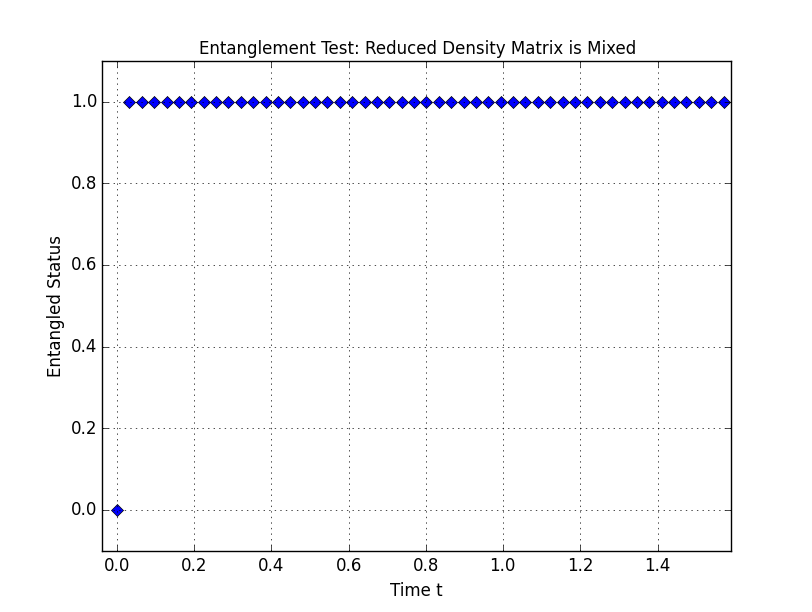
\includegraphics[scale=0.62]{figures/timeevolution-08.png}
    \caption{Checking for whether or not the reduced density matrix of the pair is mixed at various stages in the Hamiltonian evolution.\newline \texttt{0 = False = Separable,    1 = True = Entangled} }
    \label{fig: Time Evolution: Mixedness of Reduced DM}
  \end{center}
\end{figure}
\end{center}

This entanglement test has the limitation that it only works for pure states. However that is not a problem here because we are dealing with a pure state.
\par We see that the particles start getting entangled as soon as they start interacting with each other.


\pagebreak
\subsubsection{The Peres-Horodecki Criterion}
This is the plot of whether or not the state is entangled by the Peres-Horodecki criterion during all stages in its evolution. It follows the same convention: 0 represents \texttt{False} which means the state is separable; 1 represents \texttt{True} which means the state is entangled.

\begin{center}
\begin{figure}[H]
  \begin{center}
    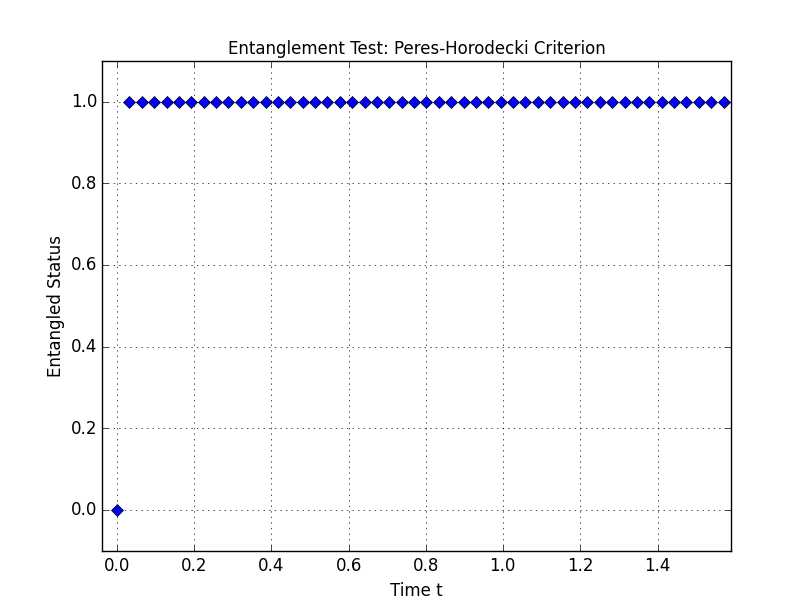
\includegraphics[scale=0.62]{figures/timeevolution-09.png}
    \caption{Checking the Peres-Horodecki criterion for entanglement at various stages in the Hamiltonian evolution.\newline \texttt{0 = False = Separable,    1 = True = Entangled}}
    \label{fig: Time Evolution: Peres-Horodecki Critetrion}
  \end{center}
\end{figure}
\end{center}

This entanglement test is more general and works well for both pure and mixed states.
\par We see that the particles start getting entangled as soon as they start interacting with each other.


\pagebreak
\subsubsection{Entropy of Entanglement and Linear Entropy of Entanglement}
The particle pair starts off with a disentangled state. Both the entropy of entanglement and the relative entropy of entanglement at time $t=0$ are zero as expected. As the state evolves and gets entangled, both of the entropies start increasing and reach their maximum values at time $t=\pi\hbar/2$. These two graphs display the trend of increase for both.

\begin{center}
\begin{figure}[H]
  \begin{center}
    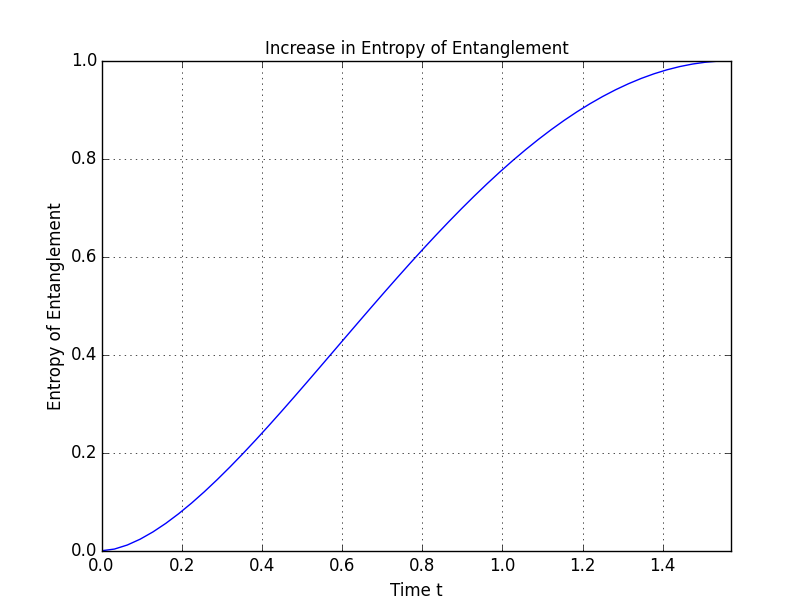
\includegraphics[scale=0.62]{figures/timeevolution-01.png}
    \caption{Increase in the entropy of entanglement of the bipartite state as it evolves under a joint Hamiltonian}
    \label{fig: Time Evolution: Entropy of Entanglement}
  \end{center}
\end{figure}
\end{center}

\begin{center}
\begin{figure}[H]
  \begin{center}
    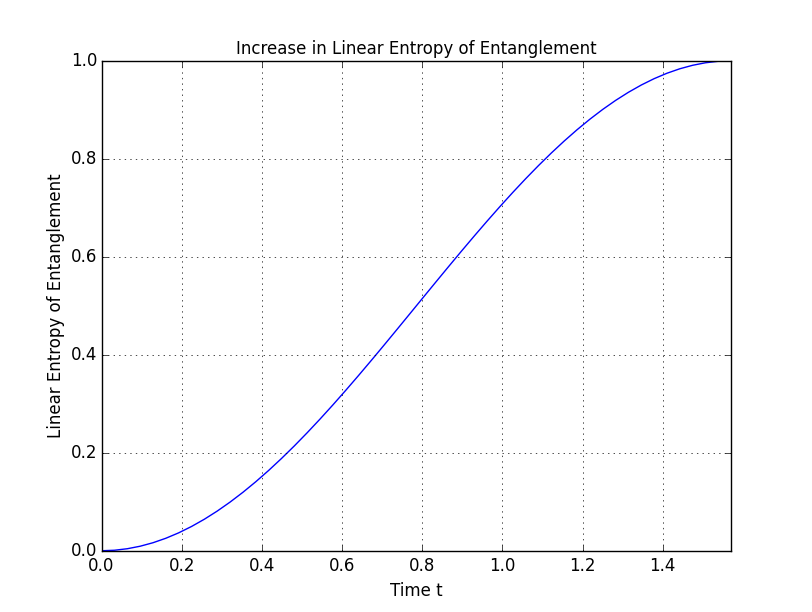
\includegraphics[scale=0.62]{figures/timeevolution-02.png}
    \caption{Increase in the linear entropy of entanglement of the bipartite state as it evolves under a joint Hamiltonian}
    \label{fig: Time Evolution: Linear Entropy of Entanglement}
  \end{center}
\end{figure}
\end{center}

The linear entropy of entanglement in this example is calculated with \texttt{normalize=True}, which normalizes it so that the completely entangled state has value 1 rather than $(1-\frac{1}{d})$ \cite{linentropybellineq}. We see that the linear entropy of entanglement closely traces the same path as the entropy of entanglement, since it is a linear approximation, and becomes 1 for the maximally entangled state.

\pagebreak
\subsubsection{Renyi Entanglement Entropies}
The Renyi entanglement entropies start with zero at the disentangled state. As the state evolves, they increase and finally reach the maximum value for the maximally entangled state.
\begin{figure}[H]
  \begin{center}
    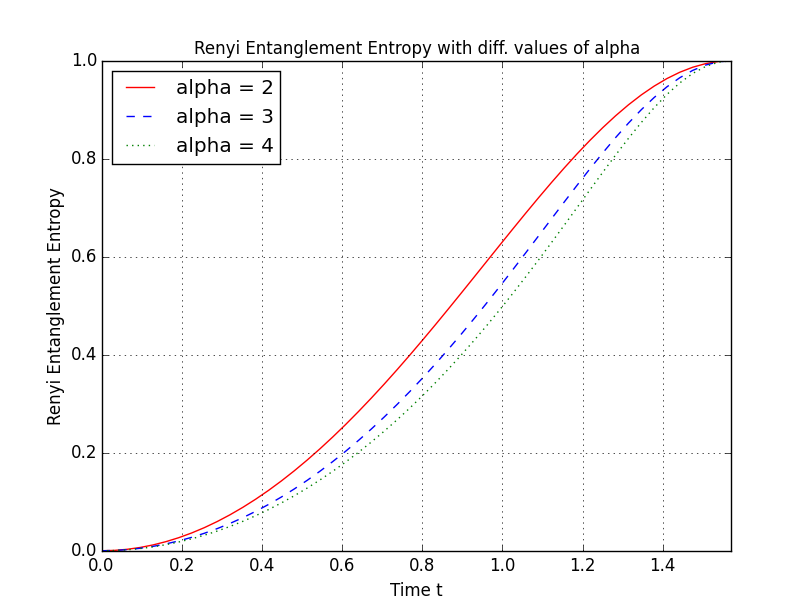
\includegraphics[scale=0.62]{figures/timeevolution-03.png}
    \caption{Increase in the Renyi entanglement entropies of the bipartite state for various values of $\alpha$}
    \label{fig: Time Evolution: Renyi Entanglement Entropies}
  \end{center}
\end{figure}

We observe that the minimum and maximum values for all values of $\alpha$ are the same: 0 and 1 respectively. With increasing value of $\alpha$, the curve shifts to the right.
\par Let us look at the Renyi entanglement entropies for a continuous range of $\alpha$ in the following 3-dimensional plot.

\begin{figure}[H]
  \begin{center}
    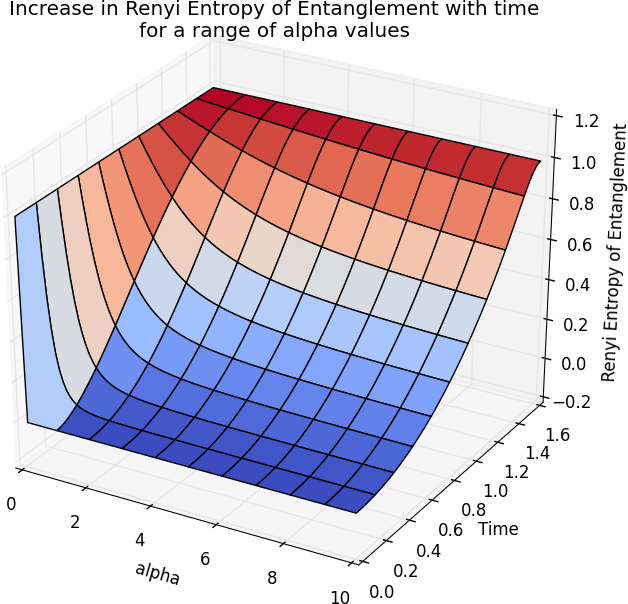
\includegraphics[scale=0.68]{figures/renyi-entg-3d.png}
    \caption{Increase in Renyi entanglement entropies with time for a range of values of $\alpha$. Time ranges from 0 to $\pi\hbar/2$ and $\alpha$ ranges from 0 to 10. Z-axis represents the Renyi entanglement entropies for all the combinations.}
    \label{fig: Time Evolution: Renyi Entanglement Entropies (3D)}
  \end{center}
\end{figure}

We observe the same trend for increasing value of $\alpha$. If we single out the curve for $\alpha=1$, we will find that it is the same as the entropy of entanglement.


\pagebreak
\subsubsection{Negativity and Logarithmic Negativity}
Negativity and logarithmic negativity both start at zero for the disentangled state. As the state evolves, they increase and reach their maximum values for the maximally entangled state.

\begin{center}
\begin{figure}[H]
  \begin{center}
    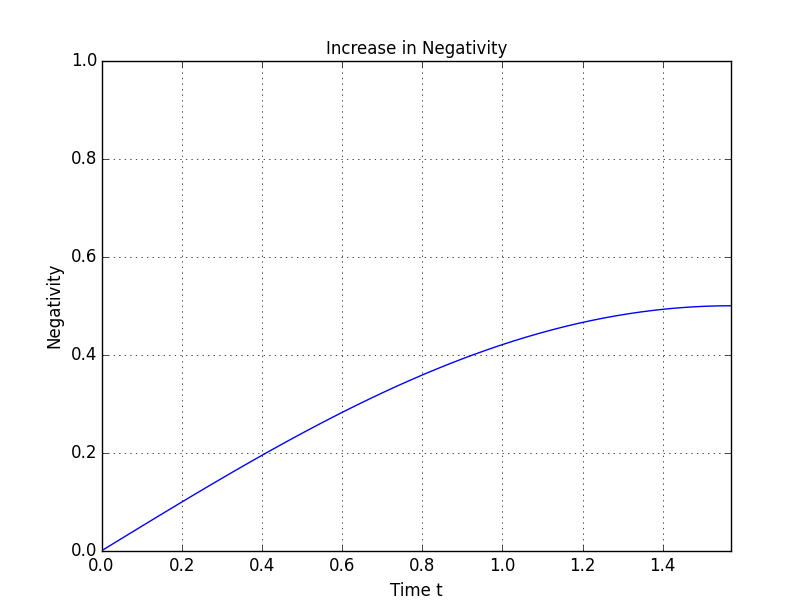
\includegraphics[scale=0.62]{figures/timeevolution-04.png}
    \caption{Increase in negativity of the bipartite state}
    \label{fig: Time Evolution: Negativity}
  \end{center}
\end{figure}
\end{center}

Negativity of the state starts at 0 when the pair is disentangled. As the state evolves, negativity gradually increases until it reaches 0.5 for the maximally entangled bipartite state.

\begin{center}
\begin{figure}[H]
  \begin{center}
    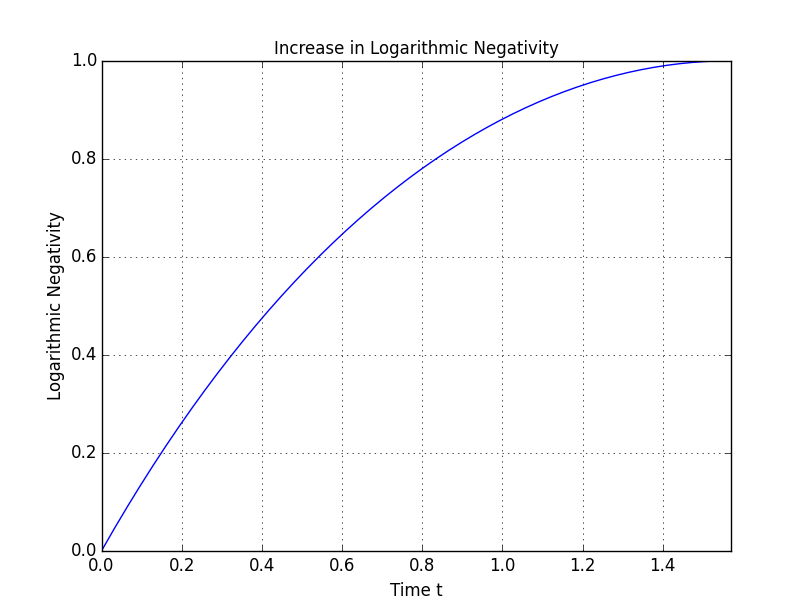
\includegraphics[scale=0.62]{figures/timeevolution-05.png}
    \caption{Increase in logarithmic negativity of the bipartite state}
    \label{fig: Time Evolution: Logaritmic Negativity}
  \end{center}
\end{figure}
\end{center}

Logarithmic negativity is an entanglement measure based on negativity that in addition has the additivity property. This plot illustrates the trend for increase in logarithmic negativity as it starts with 0 for the disentangled state and reaches a maximum value of 1 for the maximally entangled state.


\pagebreak
\subsubsection{Kullback-Leibler Distance}
The Kullback-Leibler distance can be used for defining an entanglement measure by searching over the space of all possible separable states. However here for simplicity we take a different route. We measure the KL-distance of one of the subsystems with respect to its original disentangled state to see how it changes in time. Please note that this particular graph \textit{does not} show an entanglement measure. It is just a speculative experiment.

\begin{center}
\begin{figure}[H]
  \begin{center}
    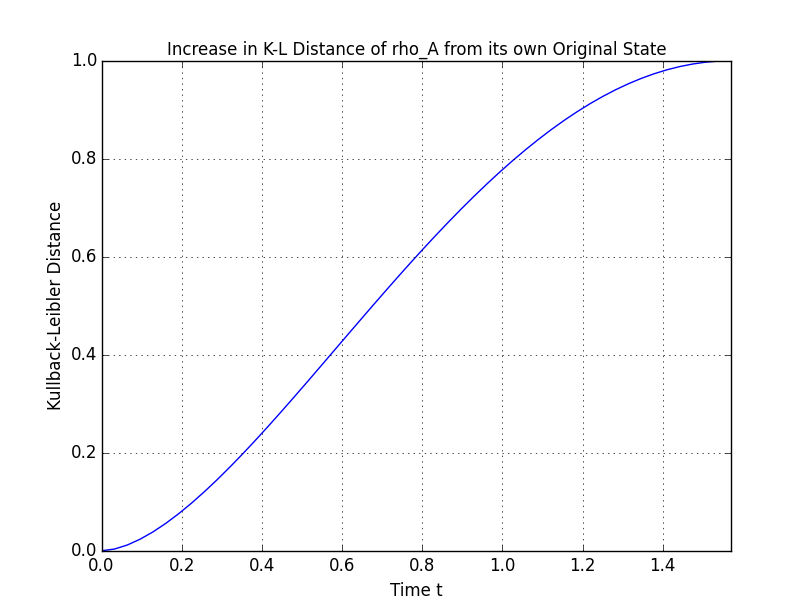
\includegraphics[scale=0.62]{figures/timeevolution-06.png}
    \caption{As the bipartite system evolves under the joint Hamiltonian, the Kullback-Leibler distance of both subsystems $\rho_A$ and $\rho_B$ with respect to their respective original states increases. This indicates that the density matrix of each subsystem is evolving and becoming different from what it was.}
    \label{fig: Time Evolution: Kullback-Leibler Distance}
  \end{center}
\end{figure}
\end{center}

To use (computationally) the Kullback-Leibler distance for defining an entanglement measure, we will have to generate the set of all possible separable states and compute the distances from our state $\rho_{AB}$ to each of them. The minimum of these distances will give the \textit{relative entropy of entanglement} for our joint density matrix $\rho_{AB}$.


\pagebreak
\subsubsection{Concurrence}
To compute concurrence, the function \texttt{concurrence} already available in QuTiP has been used. This plot illustrates the increasing trend in concurrence under the Hamiltonian evolution in question.

\begin{center}
\begin{figure}[H]
  \begin{center}
    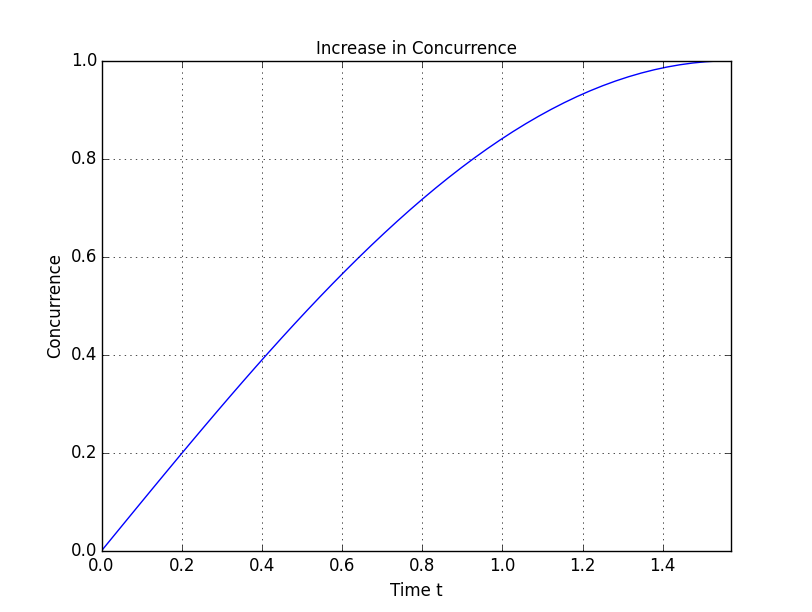
\includegraphics[scale=0.62]{figures/timeevolution-07.png}
    \caption{Increase in concurrence of the bipartite state under joint Hamiltonian evolution}
    \label{fig: Time Evolution: Concurrence}
  \end{center}
\end{figure}
\end{center}

We observe that concurrence starts with zero for the disentangled state and becomes 1 for the maximally entangled state.

\pagebreak
\subsubsection{What Happens After Time $\pi\hbar/2$?}
It should be noted that the plot upto time $\pi\hbar/2$ is not the complete picture. The system does not stay constantly at the point of maximum entanglement under this Hamiltonian evolution. We can observe changes in the amount of entanglement if we increase the time interval from $\pi\hbar/2$.
\par For example, here is the plot of concurrence from 0 to $3\pi\hbar$.

\begin{center}
\begin{figure}[H]
  \begin{center}
    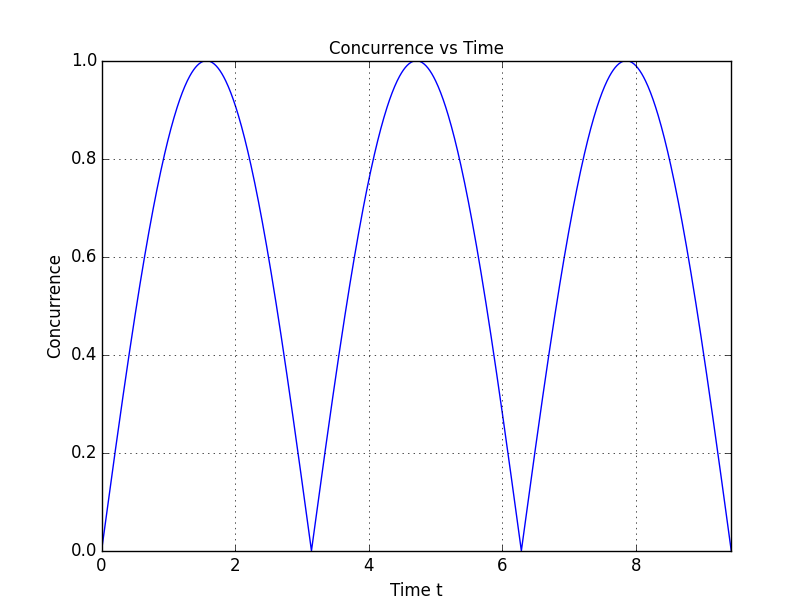
\includegraphics[scale=0.62]{figures/timeevolution-10.png}
    \caption{Concurrence as a function of time under joint Hamiltonian evolution, time ranging from 0 to $3\pi\hbar$. \newline We see that the state keeps oscillating between entangled and disentangled. At times which are multiples of $\pi\hbar$, the state becomes disentangled again.}
    \label{fig: Time Evolution: Concurrence (extended)}
  \end{center}
\end{figure}
\end{center}

\pagebreak

\subsection{Werner States}
An example of a mixed entangled state is a Werner state. Werner states are a useful test case to demonstrate the limitations of entanglement tests and measures which fail for mixed states.
\par A Werner state is defined as:
\begin{align*}
\rho_W = F \ket{\Phi^+} \bra{\Phi^+} + \frac{1-F}{3} \left( \ket{\Phi^-} \bra{\Phi^-} + \ket{\Psi^+} \bra{\Psi^+} + \ket{\Psi^-} \bra{\Psi^-} \right)
\end{align*}
where $0 \leq F \leq 1$ is the \textit{singlet fidelity}.
\par Werner states are inseparable for $F > 1/2$. We shall now see if our entanglement tests and measures work as expected on these states.

\begin{verbatim}
# -*- coding: utf-8 -*-
"""
Werner States
=============
Generate a range of Werner state with possible values of fidelity
and plot various tests and measures of entanglement

@author: Muhammad Saad
"""

from qutip import *
import numpy as np
from matplotlib import pyplot as plt
import quantinf

def werner_state(f):
    phipls = bell_state('00')
    phimns = bell_state('01')
    psipls = bell_state('10')
    psimns = bell_state('11')
    werner = ( f * phipls*phipls.dag() ) + ( ((1-f)/3) * \
             ( (phimns*phimns.dag()) + (psipls*psipls.dag()) \
             + (psimns*psimns.dag()) ) )
    return werner

fid = np.linspace(0,1)
measures = {'ent_entg':None,'neg':None,'logneg':None,'cncr':None,
            'reducedmixed':None,'phcrit':None}

for m in measures:
    measures[m] = np.zeros(len(fid))

for i in range(len(fid)):
    wrn = werner_state(fid[i])
    measures['cncr'][i] = concurrence(wrn)
    measures['ent_entg'][i] = quantinf.entropy_entg(wrn)
    measures['neg'][i] = quantinf.negativity(wrn)
    measures['logneg'][i] = quantinf.log_neg(wrn)
    measures['reducedmixed'][i] = quantinf.ismixed_reduced(wrn)
    measures['phcrit'][i] = quantinf.peres_horodecki_bipartite(wrn)

# Font size for plot
fsz = 12
# Limit for x axis
xlm = [0,1]
# Limit for y axis
ylm = [0,1]

plt.figure(1)
plt.suptitle("Tests and Measures of Entanglement on Werner States",fontsize=14)
plt.subplots_adjust(hspace=.5)

plt.subplot(321)
plt.xlabel("Fidelity",fontsize=fsz)
plt.ylabel("Concurrence",fontsize=fsz)
plt.title("Concurrence of Werner States",fontsize=fsz)
plt.plot(fid, measures['cncr'])
plt.xlim(xlm)
plt.ylim(ylm)
plt.grid(True)

plt.subplot(322)
plt.xlabel("Fidelity",fontsize=fsz)
plt.ylabel("Entr. Entanglement",fontsize=fsz)
plt.title("Entropy of Entanglement of Werner States",fontsize=fsz)
plt.plot(fid, measures['ent_entg'])
plt.xlim(xlm)
plt.ylim(ylm)
plt.grid(True)

plt.subplot(323)
plt.xlabel("Fidelity",fontsize=fsz)
plt.ylabel("Negativity",fontsize=fsz)
plt.title("Negativity of Werner States",fontsize=fsz)
plt.plot(fid, measures['neg'])
plt.xlim(xlm)
plt.ylim(ylm)
plt.grid(True)

plt.subplot(324)
plt.xlabel("Fidelity",fontsize=fsz)
plt.ylabel("Log. Negativity",fontsize=fsz)
plt.title("Logarithmic Negativity of Werner States",fontsize=fsz)
plt.plot(fid, measures['logneg'])
plt.xlim(xlm)
plt.ylim(ylm)
plt.grid(True)

xlm = [-0.04,1.02]
ylm = [-0.1,1.1]

plt.subplot(325)
plt.xlabel("Fidelity",fontsize=fsz)
plt.ylabel("Entangled Status",fontsize=fsz)
plt.title("Entanglement Test: Reduced DM is Mixed",fontsize=fsz)
plt.plot(fid, measures['reducedmixed'], 'D')
plt.xlim(xlm)
plt.ylim(ylm)
plt.grid(True)

plt.subplot(326)
plt.xlabel("Fidelity",fontsize=fsz)
plt.ylabel("Entangled Status",fontsize=fsz)
plt.title("Entanglement Test: Peres-Horodecki Criterion",fontsize=fsz)
plt.plot(fid, measures['phcrit'], 'D')
plt.xlim(xlm)
plt.ylim(ylm)
plt.grid(True)

plt.show()

\end{verbatim}

\par This program gnerates a number of plots for various entanglement tests and measures. The x-axis on all these plots represents singlet fidelity. Each value of singlet fidelity corresponds to a unique Werner state. The entanglement tests and measures are plotted as a function of the fidelity.
\par In the time evolution case from section 6.9.1, we dealt with a pure state and saw that all the tests and measures discussed so far work for pure states. However we also stressed that some of them do not work for mixed states. Some, for example, depend on the mixedness of reduced density matrix and cannot differentiate between entangled states whose reduced density matrices are mixed and states that are already mixed.
\par Werner states are a useful test case for determining which entanglement tests and measures work for mixed states. Here we take a look at some of them, starting with the ones that fail.


\subsubsection{Mixedness of Reduced Density Matrix}
This plot shows whether or not the reduced density matrix is mixed for all values of singlet fidelity for Werner states. The value 1 indicates \texttt{True} which means that the reduced density matrix is mixed. The value 0 indicates \texttt{False} which means that the reduced density matrix is pure.

\begin{figure}[H]
  \begin{center}
    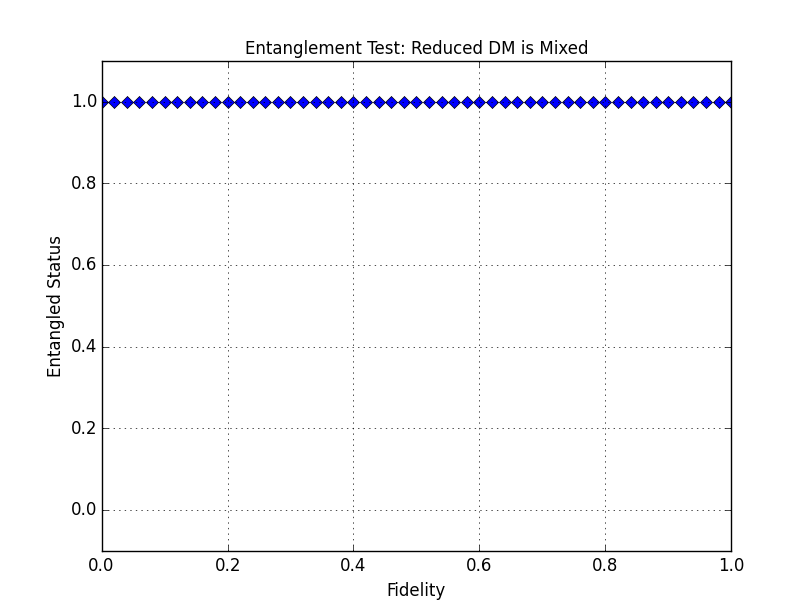
\includegraphics[scale=0.62]{figures/wernerstates-reducedmixed.png}
    \caption{Applying the entanglement test of mixedness of reduced density matrix to all possible Werner states.\newline \texttt{1 = True = Entangled,    0 = False = Separable}}
    \label{fig: Werner States: Mixedness of Reduced DM}
  \end{center}
\end{figure}

We can see that this test is failing to differentiate between separable and entangled states, showing all Werner states as entangled. This is in contrast to the time evolution example where we were dealing with a pure state. Hence we can conclude that this entanglement test is only good for pure states.

\subsubsection{Entropy of Entanglement}

\begin{figure}[H]
  \begin{center}
    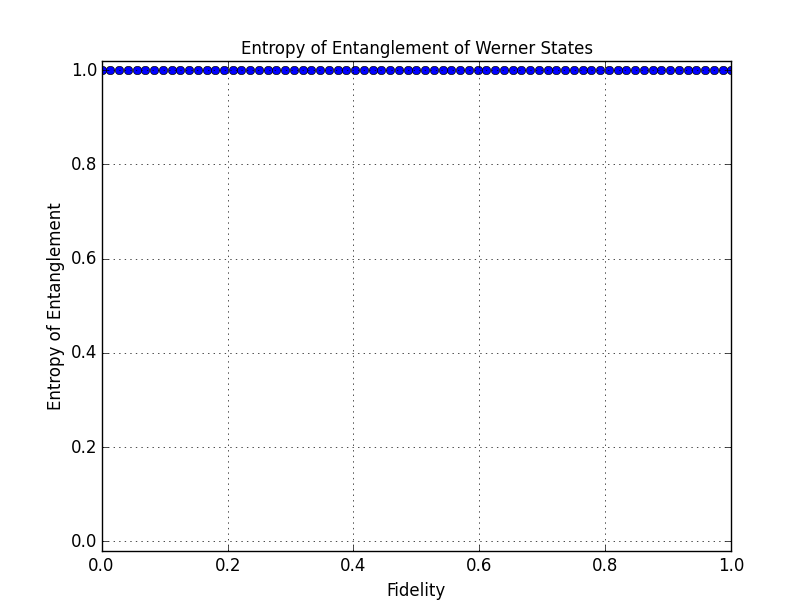
\includegraphics[scale=0.62]{figures/wernerstates-entropyentg.png}
    \caption{Entropy of Entanglement for all possible Werner states.}
    \label{fig: Werner States: Entropy of Entanglement}
  \end{center}
\end{figure}
We can see that this measure is failing to differentiate between separable and entangled states, showing maximal entanglement for all Werner states. This is due to the dependence of this measure on mixedness of the reduced density matrix, which makes it unable to identify states that are already mixed. Entropy of entanglement is good only as a measure of entanglement for pure states.
\newline
\par However, there are still a number of entanglement tests and measures that work with pure states as well as mixed states. The following are some of those tests and measures.


\subsubsection{The Peres-Horodecki Criterion}

\begin{figure}[H]
  \begin{center}
    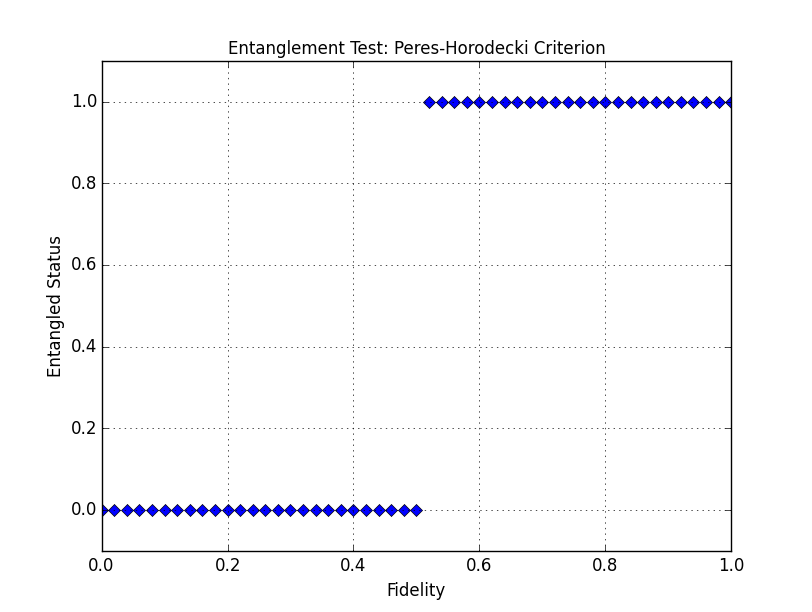
\includegraphics[scale=0.62]{figures/wernerstates-phcriterion.png}
    \caption{Applying the Peres-Horodecki criterion to all possible Werner states.\newline \texttt{1 = True = Entangled,    0 = False = Separable}}
    \label{fig: Werner States: Peres-Horodecki Criterion}
  \end{center}
\end{figure}

\par We can see that the Peres-Horodecki criterion is working as a reliable entanglement witness and showing Werner states with $F>1/2$ as entangled. It worked well for pure states in the Hamiltonian evolution case and it is also working for mixed states in the case of Werner states. This shows that the Peres-Horodecki criterion is a general entanglement witness which works well for pure as well as mixed states.


\subsubsection{Negativity and Logarithmic Negativity}

\begin{figure}[H]
  \begin{center}
    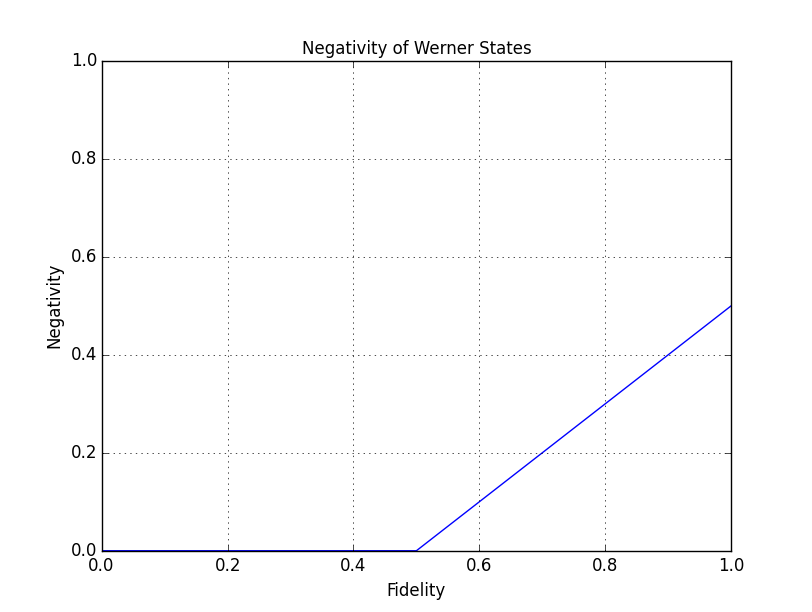
\includegraphics[scale=0.62]{figures/wernerstates-negativity.png}
    \caption{Negativity of Werner states for all possible values of singlet fidelity.}
    \label{fig: Werner States: Negativity}
  \end{center}
\end{figure}

We see that negativity starts increasing after $F=1/2$ and goes to the maximum value of 0.5 showing the state for $F=1$ as maximally entangled. This shows that negativity is a reliable measure of entanglement for both pure and mixed states.

\begin{figure}[H]
  \begin{center}
    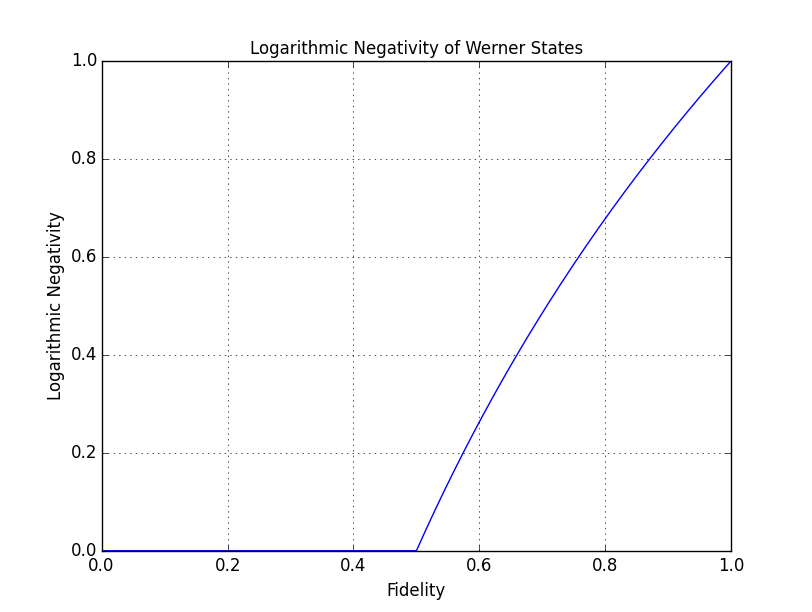
\includegraphics[scale=0.62]{figures/wernerstates-logneg.png}
    \caption{Logarithmic Negativity of Werner states for all possible values of singlet fidelity.}
    \label{fig: Werner States: Logarithmic Negativity}
  \end{center}
\end{figure}

As with negativity, logarithmic negativity also starts increasing after $F=1/2$ and reaches its maximum value for $F=1$. This shows that logarithmic negativity is also a good measure of entanglement for both pure and mixed states.


\subsubsection{Concurrence}

\begin{figure}[H]
  \begin{center}
    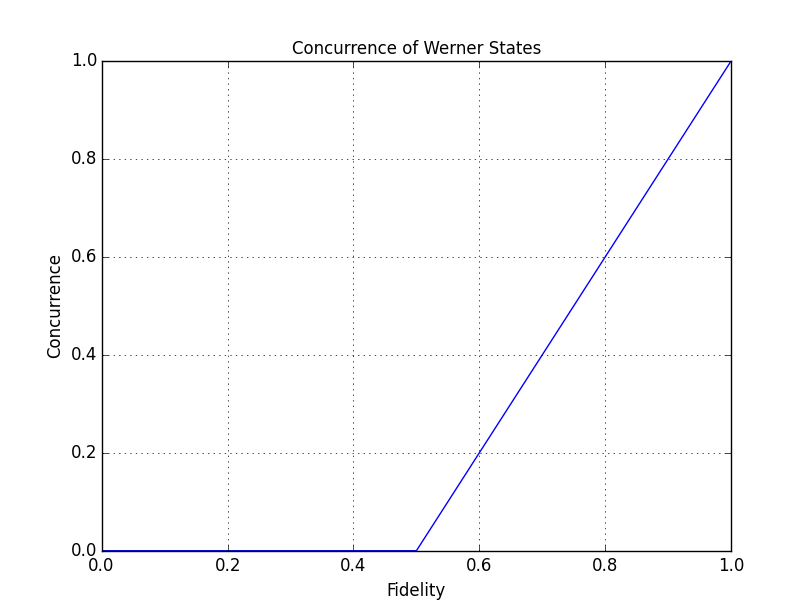
\includegraphics[scale=0.62]{figures/wernerstates-concurrence.png}
    \caption{Concurrence of Werner states for all possible values of singlet fidelity. The states start getting entangled after singlet fidelity exceeds $1/2$ and reach maximum entanglement for fidelity $F=1$.}
    \label{fig: Werner States: Concurrence}
  \end{center}
\end{figure}
We see that concurrence stays 0 for $F \leq 1/2$ when the states are disentangled. It starts increasing after $F$ exceeds $1/2$ and reaches its maximum value 1 for the maximally entangled state at $F=1$. This indicates that concurrence works for mixed states too and is a reliable measure of entanglement for both pure and mixed states.


\section{A Note About Optimizations}
QuTiP has a number of tricks available to make the functions much faster than our current implementation. However, since this project deals with the initial phase of implementing QI functions, we have not dwelled on the problem of speed optimizations. Rather we have focused primarily on implementing as many QI functions as possible. Later works on the subject can add the goal of making them faster.


\chapter{Conclusion}

In this project we explored the implementation of quantum information functions in two popular programming languages MATLAB and Python. We explored quantum information toolboxes available for both of them. After studying the advantages and limitations of both we decided to settle on Python and the Quantum Toolbox in Python (QuTiP). The successful implementation of the target functions indicates that QuTiP can serve as an excellent base for writing a quantum information toolbox.
\par MATLAB has long been dominant in the scientific programming community due to its ease of use and has gained a lot of momentum as people wrote different science and engineering toolboxes for it. Hence it has collected a huge number of very useful libraries. Its easy syntax and the availability of lots of toolboxes make it a popular choice in academia. However its license is restrictive and very expensive which makes it difficult for students and researchers to acquire a copy for their work. This also makes it an unpopular choice in industry where tough competition demands that costs be kept as low as possible.
\par Python with NumPy and SciPy on the other hand has the advantage of being completely free and open source. This makes it very attractive to the scientific programming community since science by its nature is an open process where people freely build on top of other people's work. The syntax is clearer and easier to learn. It has access to a large number of other general purpose libraries that can be used along with the scientific libraries to write more powerful programs. Python is more cross-platform than MATLAB, running on desktops, servers, mobile devices and embedded systems. This along with its non-restrictive license makes it very useful in the industry. All these advantages have been making Python increasingly popular in the scientific programming community and the number of libraries and toolboxes available for science and engineering has been growing fast.
\par However, quantum information toolboxes available for Python are fewer than there are for MATLAB \cite{quantikiqcsimulators}. The toolbox we used, QuTiP, is an excellent simulator for open quantum systems but was never designed specifically for quantum information. Hence it lacks many functions needed in quantum information theory. However we also saw that these functions can be added to QuTiP very easily and it incorporates them very well into its infrastructure. Building on top of QuTiP's well established base not only benefits the end product by eliminating a lot of development overhead, it also makes it possible for the newer functionality to be incorporated into QuTiP itself, increasing the scope of the library.
\par Over all, while writing new quantum information functions for Python is an investment of time and resources, it is an investment well worth making. Considering the advantages Python provides over MATLAB, this is the direction that will provide better results in the long term. The functions need not be written from scratch either. Functions from other toolboxes like QLib and QETLAB can be studied as a reference. Of course, this borrowing of ideas can go both ways.
\par An effort has been made in designing this document so that in the future more students from the department of physics can base their work on top of this project and add further quantum information functionality to QuTiP. A group of masters students is already working on other projects as part of which more functions will be written. These projects will study GUP-deformed and q-deformed quantum entanglement and the application of tensor networks to quantum information theory.



\nocite{*}
\printbibliography[title={References}]

\appendix
\chapter{Code: quantinf Module}

The code developed to extend QuTiP with QI functionality, all put together in a single module file. Save it with the name \texttt{quantinf.py} in order to run the time evolution and Werner states programs from chapter 6. Save the programs in the same directory as this module for convenience, if not familiar with how to add a module to the Python path.\\
A copy can be obtained from\\
https://github.com/saad440/undergrad-project \\

\begin{verbatim}
# -*- coding: utf-8 -*-
"""
This module implements a number of quantum information functions
in QuTiP (Quantum Toolbox in Python)

Project: Investigation of Entanglement Measures in QuTiP
         (IIUI, Fall 2015)

@author: Muhammad Saad <muhammad.saad@yandex.com>
"""

__all__ = ['purity','ispure','purity_of_reduced','ismixed_reduced',
        'peres_horodecki_bipartite','schmidt_decomposition', 'dist_kl',
        'entropy_entg', 'entropy_linear_entg', 'negativity', 'log_neg',
        'linear_entropy', 'entropy_renyi', 'entropy_renyi_entg' ]

from qutip import ( Qobj, ket2dm, entropy_vn, ptrace, partial_transpose )
from numpy import log2
import numpy as np

def purity(dm):
    """ Calculates trace of density matrix squared
    
    Parameters
    ----------
    dm: qobj/array-like
        Input density matrix
    
    Returns
    -------
    purity:
        Purity of the state. 1 for pure, 0.5 for maximally mixed.
    
    """
    if dm.type == 'ket':
        dm = ket2dm(dm)
    if dm.type != 'oper':
        raise TypeError("Input must be a state ket or density matrix")
    purity = (dm**2).tr()
    return purity

def purity_of_reduced(rho):
    """ Calculates trace of reduced density matrix square
    
    Parameters
    ----------
    dm: qobj/array-like
        Input density matrix
    
    Returns
    -------
    purityreduced:
        Purity of the reduced DM. 1 for pure, 0.5 for maximally mixed.
    
    """
    rhopartial = ptrace(rho,0)
    purityreduced = purity(rhopartial)
    return purityreduced

def ispure(dm):
    """ Checks whether or not a density matrix represents a pure state
    
    Parameters
    ----------
    dm : qobj/array-like
        Density operator representing the state.
    
    -------
    pure : bool
        Whether or not the state is pure. True: Pure, False: Mixed.
        
    """
    if np.round(purity(dm),8) == 1:
        return True
    else:
        return False

def ismixed_reduced(dm):
    """ One way to check for entanglement is that the reduced density
    matrix is mixed. This function checks for that criterion.
    
    Parameters
    ----------
    dm : qobj/array-like
        Density operator representing the state.
    
    -------
    mixed : bool
        Whether or not the reduced DM is mixed. True: Mixed, False: Pure
        
    """
    if np.round(purity_of_reduced(dm),8) != 1:
        return True
    else:
        return False

def schmidt_decomposition(vec):
    """ Schmidt decomposition of a bipartite vector
    Based on the implementation in QETLAB 0.9
    which was written by Nathaniel Johnston (nathaniel@njohnston.ca)
    and as of this port, last updated on December 1, 2012
    
    Parameters
    ----------
    vec : qobj, ket vector of product state
        ket vector representing the bipartite state
    
    -------
    Returns:
    [s, u, v]
    s : list of floats
        Schmidt coefficients
    u : list of Qobj
        list of left Schmidt vectors of ket
    v : list of Qobj
        list of right Schmidt vectors of ket
        
    """
    if vec.type != 'ket':
        raise TypeError("Input must be a ket vector.")
    if len(vec.dims[0])==1:
        raise TypeError("Input must be a joint state.")
    
    dim = vec.dims[0][0]
    vecnp = vec.full()
    vecnpr = np.reshape(vecnp,[dim,dim])
    um,s,vm = np.linalg.svd(vecnpr)
    
    s = list(s)
    
    def extract_vecs(mat):
        veclist = list()
        for j in range(mat.shape[1]):
            veclist.append(Qobj(mat[:,j]))
        return veclist
    u = extract_vecs(um)
    v = extract_vecs(vm)
    
    return [s,u,v]

def peres_horodecki_bipartite(rho, mask=[0,1]):
    """ Tests the given bipartite state for Peres-Horodecki criterion
    
    Parameters
    ----------
    rho: qobj/array-like
        Density operator for the state
    mask: list of int, length 2
        mask used for partial transpose
    
    Returns
    -------
    isentangled: bool
        True for entangled, False for disentangled
    
    """
    if rho.type != 'oper':
        raise TypeError("Input must be a density matrix")
    rhopt = partial_transpose(rho,mask)
    rhopt_eigs = rhopt.eigenenergies()
    if min(rhopt_eigs) < 0:
        isentangled = True
    else:
        isentangled = False
    return isentangled

def entropy_entg(rho, base=2):
    """ Calculates the entropy of entanglement of a density matrix
    
    Parameters:
    -----------
    rho : qobj/array-like
        Input density matrix
    base:
        Base of log
    
    Returns:
    --------
    ent_entg: Entropy of Entanglement
    
    """
    if rho.type == 'ket':
        rho = ket2dm(rho)
    if rho.type != 'oper':
        raise TypeError("Input must be density matrix")
    rhopartial = ptrace(rho,0)
    ent_entg = entropy_vn(rhopartial,base)
    return ent_entg

def linear_entropy(dm, normalize=False):
    """ Returns the linear entropy of a state.
    
    Parameters
    ----------
    dm : qobj/array-like
        Density operator representing the state.
    normalize : bool
        Optional argument to normalize linear entropy such that the
        completely mixed state has LE = 1 rather than 1-1/d. [1]
        Default: False
    
    ----------
    le : float
        Linear entropy
    
    ----------
    References:
        [1] "Linear entropy and Bell inequalities", Santos and Ferrero,
            Phys. Rev. A 62, 024101
    
    """
    if dm.type not in ('oper','ket'):
        raise TypeError("Input must be a Qobj representing a state.")
    if dm.type=='ket':
        dm = ket2dm(dm)
    
    le = 1 - (dm**2).tr()
    if normalize:
        d = dm.shape[0]
        le = le * d/(d-1)
    return le

def entropy_linear_entg(rho, normalize=True):
    """ Calculates the linear entropy of entanglement of a density matrix
    
    Parameters:
    -----------
    rho : qobj/array-like
        Input density matrix
    
    Returns:
    --------
    linent_entg: Linear Entropy of Entanglement
    
    """
    if rho.type == 'ket':
        rho = ket2dm(rho)
    if rho.type != 'oper':
        raise TypeError("Input must be density matrix")
    rhopartial = ptrace(rho,0)
    linent_entg = linear_entropy(rhopartial,normalize)
    return linent_entg

def entropy_renyi(rho,alpha):
    """ Calculate Renyi entropy of the density matrix with given index
    (Currently limited to 2-level systems)
    
    Parameters
    ----------
    dm: qobj/array-like
        Input density matrix
        
    alpha: Renyi index alpha
    
    Returns
    -------
    ent_rn: Renyi Entropy
    
    """
    if rho.type != 'oper':
        raise TypeError("Input must be a density matrix")
    qi = rho.eigenenergies()
    
    if alpha == 1:
        ent_rn = entropy_vn(rho,2)
    elif alpha >= 0:
        ent_rn = ( 1/(1-alpha) ) * log2 ( sum( qi**alpha ) )
    else:
        raise ValueError("alpha must be a non-negative number")
    return ent_rn

def entropy_renyi_entg(rho,alpha):
    """ Calculate Renyi entropy of entanglement for the DM with given index
    (Currently limited to 2-level systems)
    
    Parameters
    ----------
    dm: qobj/array-like
        Input density matrix
        
    alpha: Renyi index alpha
    
    Returns
    -------
    ent_rn_entg: Renyi Entropy of Entanglement
    
    """
    rhopartial = ptrace(rho,0)
    ent_rn_entg = entropy_renyi(rhopartial,alpha)
    return ent_rn_entg

def negativity(rho,mask=[1,0]):
    """ Calculate the negativity for a density matrix
    
    Parameters:
    -----------
    rho : qobj/array-like
        Input density matrix
    
    Returns:
    --------
    neg : Negativity
    
    """
    if rho.type != 'oper':
        raise TypeError("Input must be a density matrix")
    rhopt = partial_transpose(rho,mask)
    neg = ( rhopt.norm() - 1 ) / 2
    return neg

def log_neg(rho,mask=[1,0]):
    """ Calculate the logarithmic negativity for a density matrix
    
    Parameters:
    -----------
    rho : qobj/array-like
        Input density matrix
    
    Returns:
    --------
    logneg: Logarithmic Negativity
    
    """
    if rho.type != 'oper':
        raise TypeError("Input must be a density matrix")
    rhopt = partial_transpose(rho,mask)
    logneg = log2( rhopt.norm() )
    return logneg

def dist_kl(rho, sgm):
    """ Calculates the Kullback-Leibler distance (a.k.a. relative entropy)
    between DMs rho and sgm representing two-level systems.
    
    Parameters
    ----------
    rho : qobj/array-like
        First density operator.

    sgm : qobj/array-like
        Second density operator.

    Returns
    -------
    kldist : float
        Relative Entropy between rho and sgm.
    
    """
    if rho.type != 'oper' or sgm.type != 'oper':
        raise TypeError("Inputs must be density matrices..")
    
    ent_vn = entropy_vn(rho,2)
    
    r_eigs = rho.eigenenergies()
    s_eigs = sgm.eigenenergies()
    # too small negtive values may give trouble
    s_eigs = np.round(s_eigs,8)
    
    kldist = -ent_vn
    for pj, qj in zip(r_eigs,s_eigs):
        if qj==0:
            pass
        else:
            kldist -= pj * log2(qj)
            
    kldist = abs(kldist)
    return kldist

\end{verbatim}


\chapter{Code: Numerical Solver}

Some extra bits of code to help check if a bipartite state's ket vector can be separated numerically.\\
A copy can be obtained from\\
https://github.com/saad440/undergrad-project 

\begin{verbatim}
# -*- coding: utf-8 -*-
"""
This module contains simple solver functions to check if a given state
ac|00>+ad|01>+bc|10>+bd|11> is separable and if it is, solve for a,b,c,d.

Project: Investigation of Entanglement Measures in QuTiP
         (IIUI, Fall 2015)

@author: Muhammad Saad <muhammad.saad@yandex.com>
"""

__all__ =  ['solve_coefficients', 'verify_separability',
            'is_separable_coeffs', 'is_separable']

from scipy.optimize import fsolve
import numpy as np

def solve_coefficients(coeffprod):
    """ Simple solver to separate a,b,c,d from products ac,ad,bc,bd
    
    Parameters
    ----------
    coeffprod : list
                [ac,ad,bc,bd] of which to separate a, b, c and d.
    
    -------
    z :       list
                The solutions [a,b,c,d]

    Examples
    --------
    >>> 
    
    """
    ac,ad,bc,bd = coeffprod
    def f(x):
        a,b,c,d = x
        r = np.zeros(4)
        r[0] = a*c - ac
        r[1] = a*d - ad
        r[2] = b*c - bc
        r[3] = b*d - bd
        return r
    z = fsolve(f,[1,1,1,1])
    return z

def verify_separability(coeffprod,coeffsepd,tol=6):
    """ Verify that the solutions obtained are actually valid
    
    Parameters
    ----------
    coeffprod : list
                [ac,ad,bc,bd] of which to separate a, b, c and d.
    coeffsepd : list
                [a,b,c,d], the solutions obtained from solve_coefficients
    
    -------
    vrfy :      bool
                True: match, False: donot match
    
    """
    a,b,c,d = coeffsepd
    ac,ad,bc,bd = coeffprod
    vrfy = [np.round((a*c-ac),tol)==0, np.round((a*d-ad),tol)==0,
            np.round((b*c-bc),tol)==0, np.round((b*d-bd),tol)==0]
    if all(vrfy):
        return True
        
def is_separable_coeffs(coeffprod,tol=6):
    """ Check whether a list of coefficients to a state is separable
    
    Parameters
    ----------
    coeffprod : list
                [ac,ad,bc,bd] of which to separate a, b, c and d.
    tol :       int
                rounding error tolerance
    
    -------
    separable : bool
                True: Coefficients are separable, False: not separable
    
    """
    ac,ad,bc,bd = coeffprod
    a,b,c,d = solve_coefficients(coeffprod)
    coeffsepd = a,b,c,d
    separable = verify_separability(coeffprod,coeffsepd)
    return bool(separable)
    
def is_separable(kt,tol=6):
    """ Check whether a state vector represents a separable state
    Note: Currently limited to 2-level product states of two particles
    
    Parameters
    ----------
    kt  :       ket state vector
                [ac,ad,bc,bd] of which to separate a, b, c and d.
    tol :       int
                rounding error tolerance
    
    -------
    separable : bool
                True: State is separable, False: not separable
    
    """
    # Current limitations. Need to generalize
    limitations = [ kt.isket, kt.shape==[4,1] ] # kt.dims==[[2,2],[1,1]]
    if not all(limitations):
        raise ValueError("Currently limited to 2-level product states of 2 particles")
    ac,ad,bc,bd = kt.full()
    ac,ad,bc,bd = ac[0],ad[0],bc[0],bd[0]
    coeffprod = ac,ad,bc,bd
    is_sp = is_separable_coeffs(coeffprod,tol)
    return is_sp
\end{verbatim}



\end{document}

